% File: tex/ics.tex
% Author: Timo L. R. Halbesma <timo.halbesma@student.uva.nl>
% Version: 0.01 (Initial)
% Date created: Sat Oct 24, 2015 12:28 am
% Last modified: Thu Sep 01, 2016 06:52 PM
%
% Description: Master's thesis, Theory


\documentclass[MScProj_TLRH_ClusterEnergy.tex]{subfiles}
\begin{document}

\chapter{From X-ray Constrains to Initial Conditions}
\label{sec:constrains}

\section{Multi-Wavelength Observational Campaign}
\label{sec:wisecampaign}
The X-ray study of \citet{2014cxo..prop.4448W} aims to investigate AGN feedback 
in the merging cluster of galaxies Cygnus~A. This approved \satellite{Chandra} 
proposal titled `The Rise to Power: half a billion years of intense AGN activity 
in the Merging Cluster Cygnus~A' is part of an ongoing multi-wavelength campaign
together with radio observations of the region surrounding the Cygnus galaxy 
TODO: ask Michael for radio references. 
The final product will comprise a staggering 2.2 mega second observation. The
first mega second of data has been acquired, and first-results will soon be 
published \citep[in prep]{2016MNRAS.123..456W}. Upon completion by the end of 
2017, the new exposure combined with 232~ksec archival data will be the deepest
X-ray observation of any merging cluster of galaxies to date, to our knowledge. 
These data allow us to infer initial conditions to set up numerical simulations
of the merger using the proprietary code \code{Toycluster} published by
\citet{2014MNRAS.438.1971D}, \citet[in prep]{2016MNRAS.000.000D}. In short, the 
system is set up without the AGN as an idealised, binary merger of an ideal
smoothed particle hydrodynamics gas in a potential dominated by collisionless
dark matter. A detailed description is presented in chapter~\ref{sec:methods}.
In this chapter we describe how the input parameters for the code are obtained
from the X-ray data shown in section~\ref{sec:xray}. In 
section~\ref{sec:results-xray} we present $\beta$-model 
(equation~\eqref{eq:betamodel}) fits to the hot intra cluster medium observed
by \satellite{Chandra}, which gives the central gas number density $n_0$ 
and the core radius $r_c$. The total mass is inferred under the assumption of a
fixed baryon fraction (17 per cent) at the virial radius and by adopting the 
Hernquist dark matter density profile (equation~\eqref{eq:hernquist}). The mass
estimates of the sub clusters is presented in section~\ref{sec:gas-to-dm}. This
gives sufficient observational constrains to set up initial conditions for the 
numerical simulations presented in chapter~\ref{sec:sim}.


% \textbf{Stolen from Michael's Chandra Proposal}
% 
% From ``The Rise to Power: Half a Billion Years of Intense AGN Activity in the
% Merging Cluster Cygnus~A'' we obtain the following regarding the merger,
% including interesting references.
% 
% ``Finally, on the largest scales, the sub-cluster containing Cygnus~A is
% undergoing a nearly equal mass merger that is driving a shock into the outer
% cluster atmosphere and could be contributing to the high level of AGN activity
% observed \citep{2002ApJ...565..195S, 1997ApJ...488L..15O, 1999ApJ...521..526M,
% 2005AJ....130...47L, 2013AN....334..346S, 2016MNRAS.123..456W}'' \\
% 
% 
% ``Existing Chandra observations reveal a pronounced surface brightness
% discontinuity, roughly elliptical in shape, and surrounding the radio source in
% Cygnus~A (see Fig. 1). This discontinuity has been interpreted as the cocoon
% shock inferred by \citep{1988ApJ...334L..73C} and studied previously by
% \citep{2006ApJ...644L...9W}, who derived a Mach number of \mytilde 1.3 and a
% total kinetic power of \mytilde $1 \times 10^{46}$ erg s$^{-1}$ . Similar values
% of M \mytilde 1.37 and \mytilde$4 \times 10^{45}$ ergs$^{-1}$ were obtained by
% \citep{2015IAUS..313..236N} from fits to a spherically symmetric shock model. An
% analysis of the azimuthal variation in the shock yields a range of Mach values
% from \mytilde $1.2 - 1.8$ \citep{2016MNRAS.123..456W} and may reflect
% asymmetries in the environment of Cygnus~A due to ``cluster weather''
% \citep{2005ApJ...630..740B, 2010MNRAS.407.1277M} or precession of its jets
% \citep{2006MNRAS.373L..65H}. Spectral mapping based on the existing 232 ksec
% archival Chandra data has also revealed evidence for a temperature jump in the
% ICM associated with the shock edge and consistent with the Mach values
% determined from the surface brightness \citep{2016MNRAS.123..456W}.'' \\
% 
% ``Unfortunately, the current data does not detect the temperature jump around
% the full circumference of the shock, but only at the leading edges close to the
% hotspots and the binning required to achieve a significant detection precludes
% resolving the shock temperature structure in detail. Nonetheless, these results
% clearly indicate that the cocoon shock in Cygnus~A is depositing a significant
% amount of energy into the surrounding cluster gas and provides a good estimate
% for the mean jet power during the current outburst of Cygnus~A. The requested
% deeper image will resolve the shock front itself on \mytilde $1-2$ kpc scales
% and at \mytilde 30 positions distributed angularly around the shock boundary,
% especially in the region of the hotspots. It will also be possible to measure
% temperature jumps along small sections of the front, to verify that it is a
% predominantly hydrodynamic shock.'' \\
% 
% ''On the scale of the merging system itself, the ICM surrounding Cygnus~A shows
% an asymmetric morphology with an extension in the X-ray emission roughly aligned
% with the major axis in the radio galaxy. This asymmetry has been noted
% previously \ref{2002ApJ...565..195S} and extends to well over \mytilde 200 kpc
% from the center of Cygnus~A (see Fig. 2). Its origin is unclear, but may
% represent cluster gas that has been displaced and compressed by relativistic
% material that has passed through the hot spots at the ends of the jets.
% Similarly, a dramatic filamentary structure roughly \mytilde 280 kpc $\times$ 60
% kpc is clearly seen located between the two merging sub-clusters at a radius of
% \mytilde $300 - 400$ kpc and exhibits a temperature of ~ 9 keV, albeit with
% large uncertainties again due to the low surface brightness. This filament falls
% within the interstitial shock region between the two merging sub-clusters in
% Cygnus~A and is consistent with the temperature jump associated with this region
% detected in lower spatial resolution data \citep{1999ApJ...521..526M,
% 2013AN....334..346S, 2016MNRAS.123..456W}. Mass estimates for the NW sub-cluster
% imply that Cygnus~A is undergoing a 2:1 mass merger; however, this sub-cluster
% is very far off-axis in the current dataset and the effective exposure is low
% making the mass ratio determination uncertain. Dynamical modelling of the system
% favours a timeframe for the merger \mytilde 0.5 Gyr prior to core passage
% \citep{2005AJ....130...47L}.''\\

% ``Taken together, these features imply a dynamic environment surrounding Cygnus~A over the past ~ 500 Myr. The proposed deeper exposure will provide accurate
% estimates for the energetics of these features and constrain variations in the
% energy output of Cygnus~A on timescales ~ 300 Myr. At the same time, we will
% derive better constraints on the merger itself, in particular the mass ratio and
% associated shock, to study how this ongoing merger has affected activity in
% Cygnus~A over the past ~ 1 Gyr.'' \\
% 
% ``As the Faraday RM is proportional to the integral of the line-of-sight
% magnetic field weighted by the thermal electron density, an accurate 3D model of
% the density from X-ray observations is vital to deduce field strengths.'' -- But
% this is at 30 kpc, right? \\

% \textbf{End of `Stolen from Michael's Chandra Proposal'}

\section{X-ray Surface Brightness Maps}
\label{sec:xray}
We begin this chapter by showing the amazing data. The ICM of Cygnus~A, referred
to as `CygA', is centered at $(19:59:28.25,+40:44:02.85)$. This centroid 
coincides with the center of the classical radio double at $(19:59:28.359, 
+40:44:02.07)$, obtained from the fits file of the \citet{1996A&ARv...7....1C}
JVLA observation at 5~GHz. Contours of this observation are overplotted on
the core region of CygA in Figure~\ref{fig:CygA_Xray}. Hot spots in the X-ray
contours do correspond to radio hot spots but, interestingly, the jest believed
to have created these distinct features appear to be misaligned at different
wavelengths. Increasing the field of view in Figure~\ref{fig:CygA_Xray_extended}
shows a beautiful mosaic of the extended emission in the Cygnus cluster. The
sub cluster, referred to as `CygB', appears to the North West of CygA only
after smoothing a log stretch of the surface brightness with, in this case a
$9$~pixel radius, Gaussian to enhance this less luminous structure. The center
of CygB is at $(19:58:46.15,+40:54:01.15)$. The particular choice of colour 
stretch in the figure, however, fully saturates the core region. The radio source
is located within this saturated region. A slightly different stretch is chosen
in Figure~\ref{fig:ruler} to show the disturbed X-ray medium of the core region
inside the larger cluster region. The field-of-view here is smaller than in the
figure showing the full mosaic, and a ruler has been added to measure the 
distance between both haloes. This is an important quantity to select the 
simulation snapshot that best-represents the observation later on.

\begin{figure}
\centering
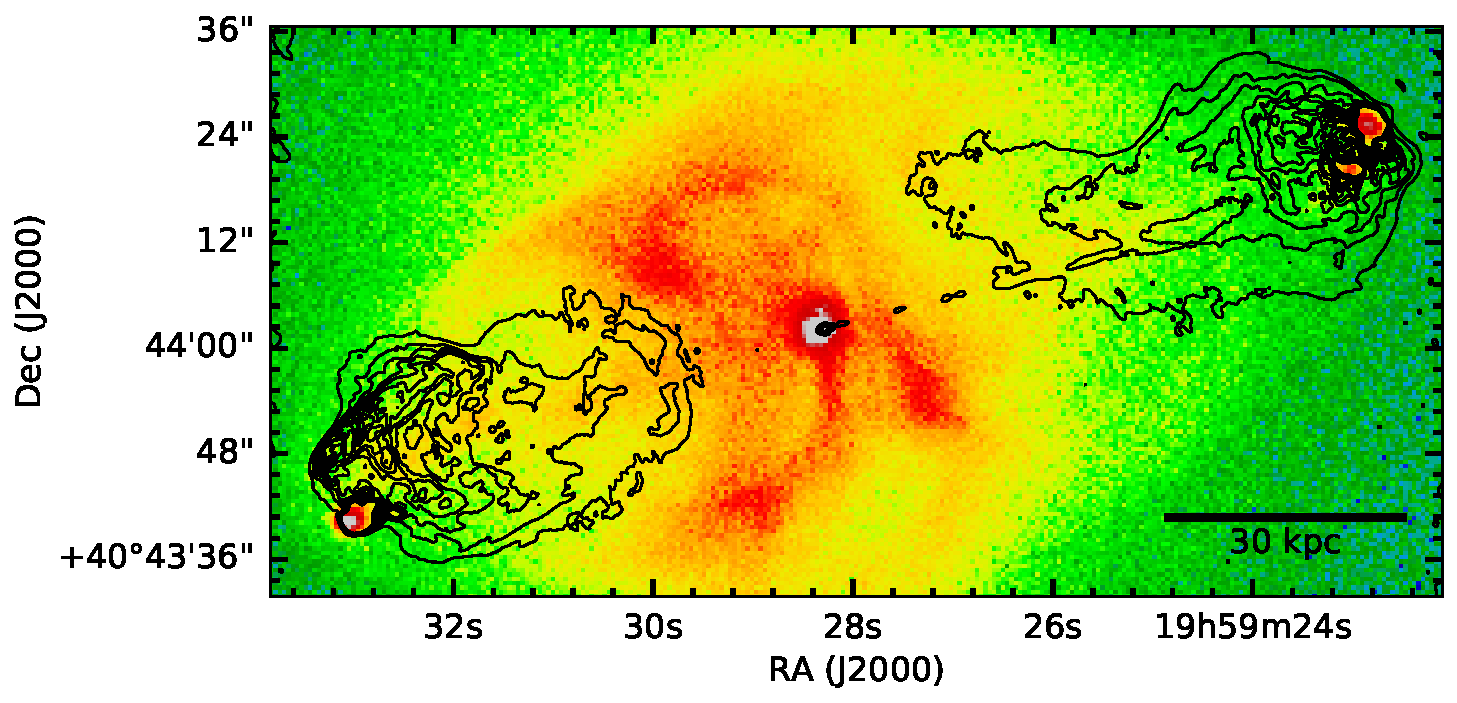
\includegraphics[width=\textwidth]{ics/xray/CygA_Radio_5GHz.pdf}
\caption{Preliminary 982.05 ksec \satellite{Chandra} X-ray observation of the 
         central region of Cygnus~A \citep[in prep]{2016MNRAS.123..456W}
         with 5~GHz, 0.5'' resolution JVLA contours overlay
         \citep{1996A&ARv...7....1C}. The radio hotspots correspond to X-ray
         hot spots at the jet terminus, and several hot spots and X-ray cavities
         are visible surrounding the central region where no radio emission is
         seen. A slight misalignment is seen between the radio and the X-ray
         jet.
         }
\label{fig:CygA_Xray}
\end{figure}

\begin{figure}
\centering
\makebox[\textwidth][c]{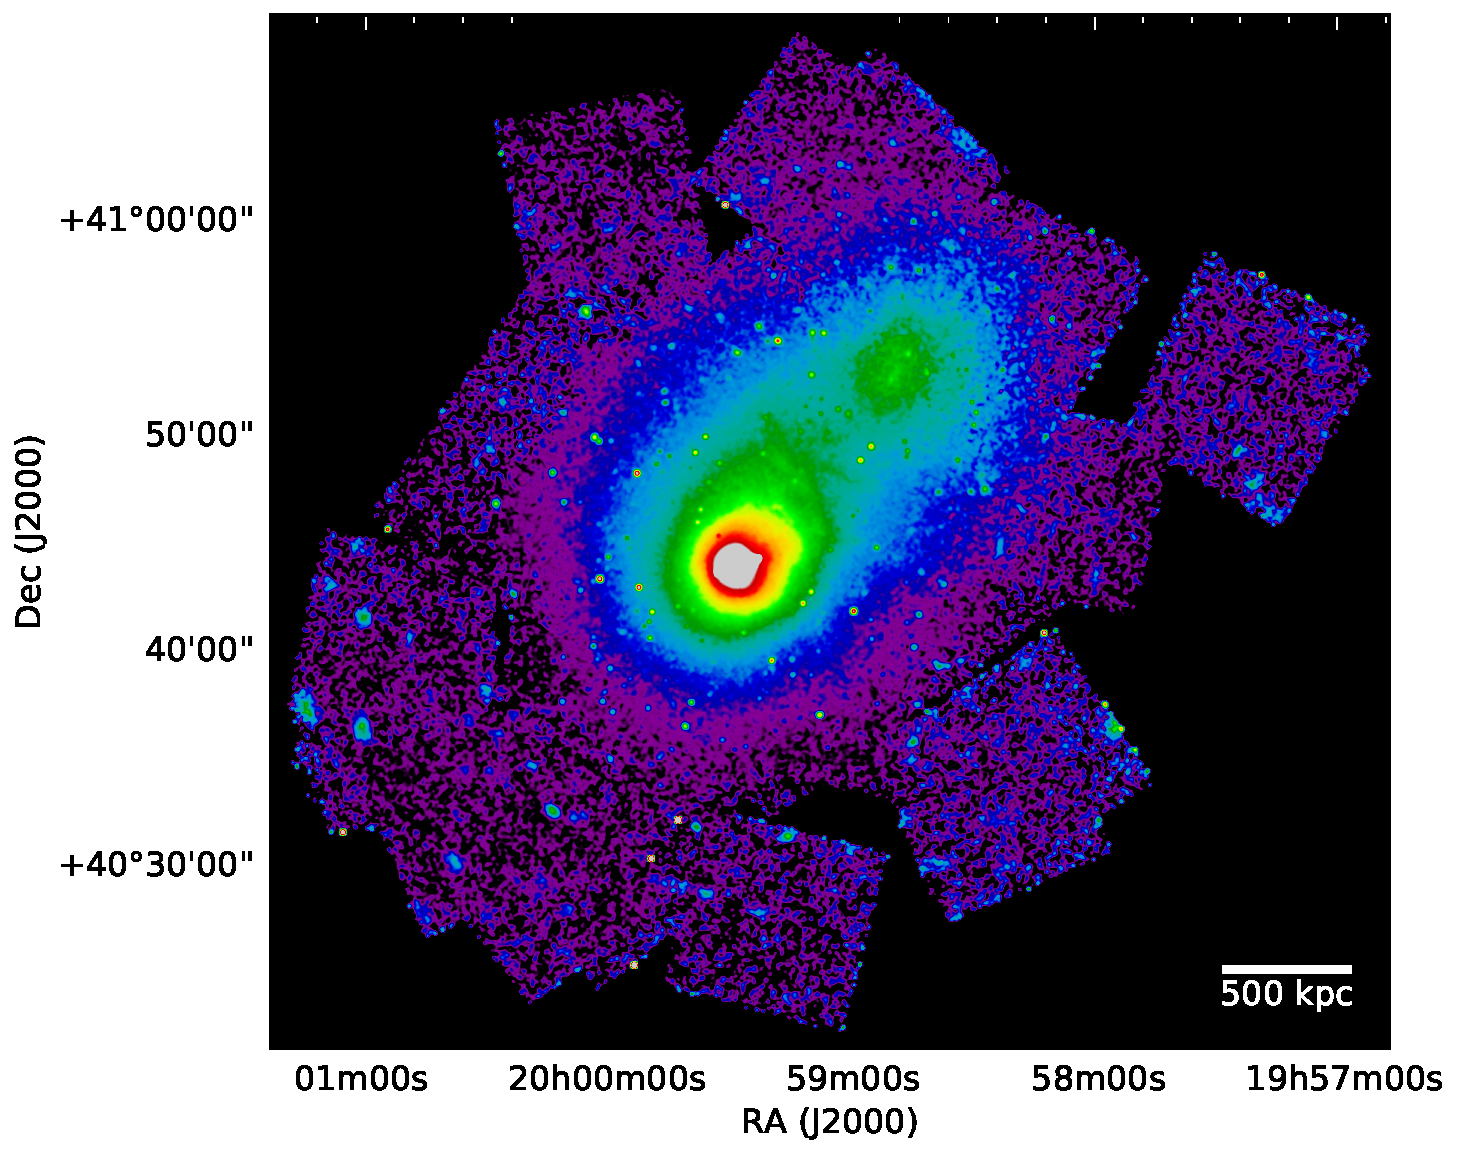
\includegraphics[width=1.3\textwidth]{ics/xray/cygnus_mosaic.pdf}}%
\caption{Preliminary 982.05 ksec \satellite{Chandra} X-ray observation of the 
         full mosaic showing the extended emission surrounding Cygnus~A
         \citep[in prep]{2016MNRAS.123..456W} smoothed with a 9 pixel radius.
         The radio source is located in the saturated region.
         }
\label{fig:CygA_Xray_extended}
\end{figure}

\begin{figure}
\centering
\makebox[\textwidth][c]{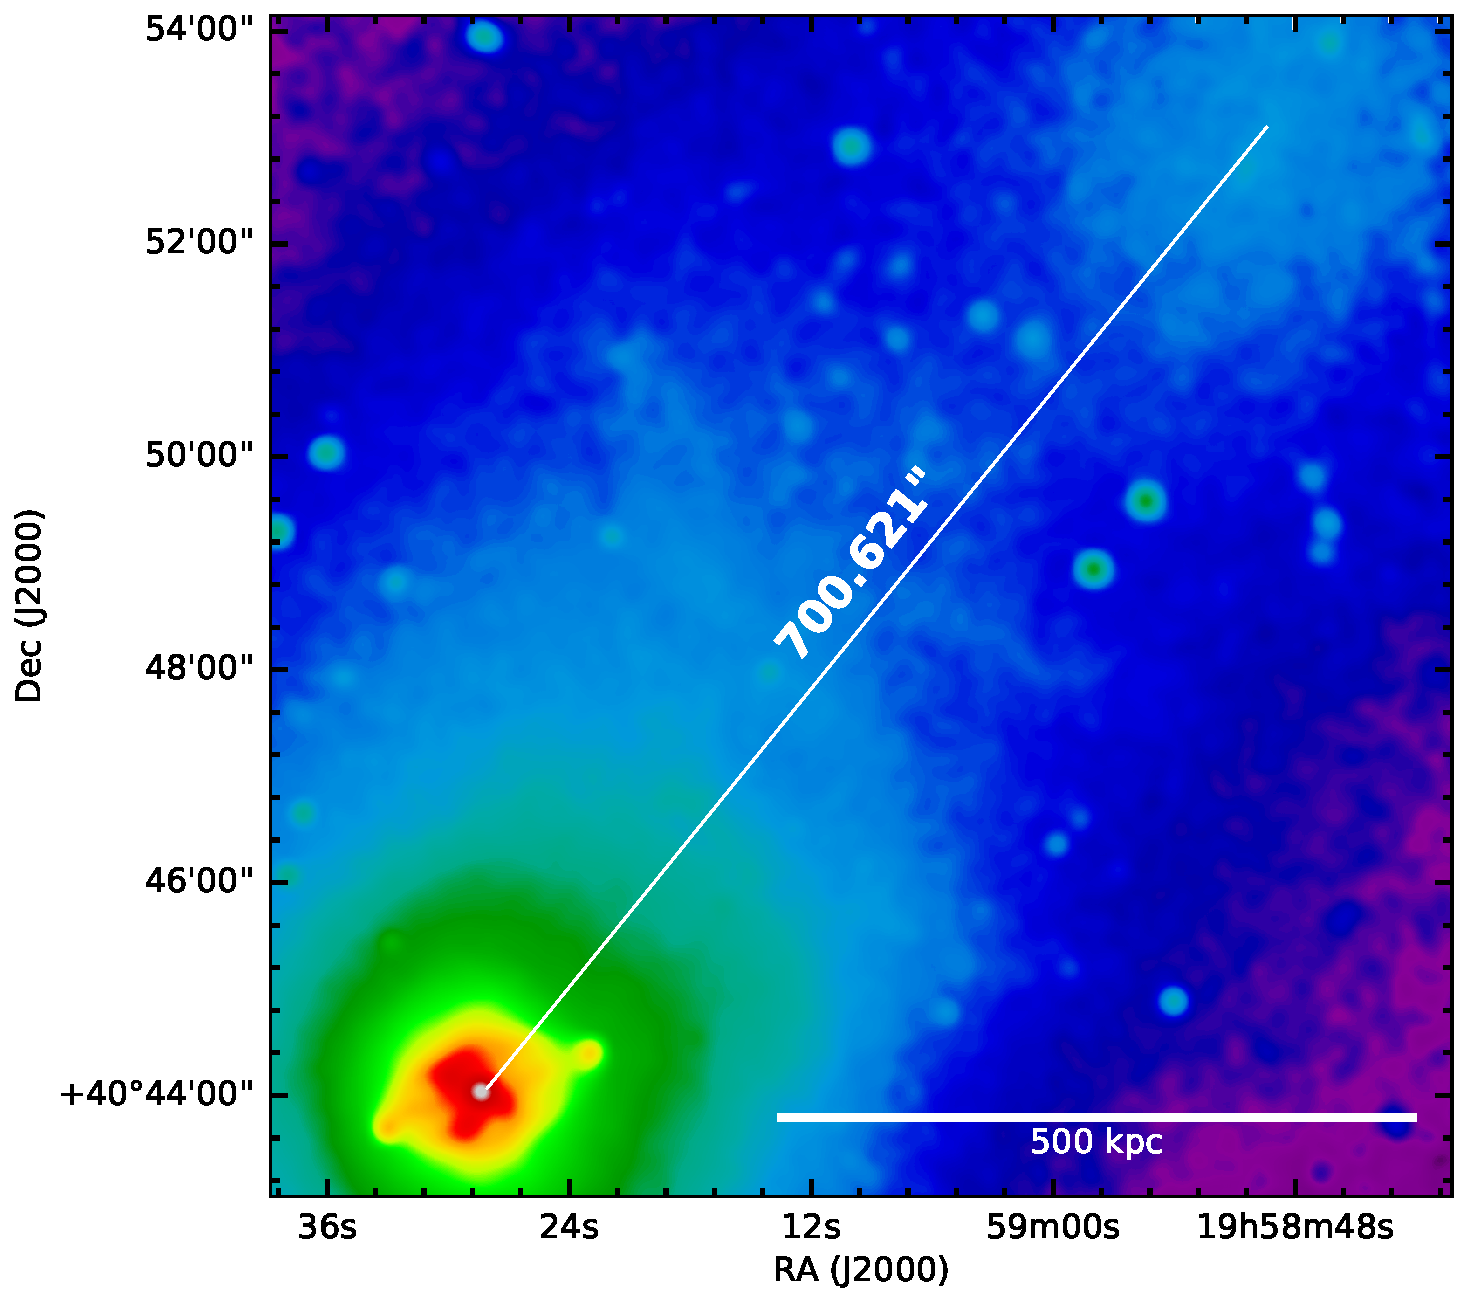
\includegraphics[width=1.2\textwidth]{ics/xray/mosaic_xray_ruler.pdf}}%
\caption{Preliminary 982.05 ksec \satellite{Chandra} X-ray observation of the 
         extended emission surrounding Cygnus~A \citep[in prep]{2016MNRAS.123..456W}
         zoomed in on both sub clusters. The stretch is chosen to show the 
         morphology of the core region, albeit smoothed with a 9 pixel Gaussian.
         A ruler is added to show the observed projected core separation between
         CygA and CygB.
         }
\label{fig:ruler}
\end{figure}



\section{Radial Profiles: Number Density}
\label{sec:numberdensity}
We continue with a consideration of ICM properties of both sub clusters. In 
particular, we would like to show that the clusters can be modelled as a coronal 
plasma (as presented in section~\ref{sec:clustergas}), and we discuss validity 
of the fluid approximation which is a requirements to use Smoothed Particle 
Hydrodynamics. Details of the numerical implementation to model the gas as SPH
particles are resented in section~\ref{sec:methods-gadget}.

Recall that we need to show that the cooling timescale is both larger than the
age of the cluster, and larger than the timescale for Coulomb interactions 
$t_{\text{cool}} >> t_{eq}$ such that the plasma follows the Maxwell-Boltzmann 
distribution. First, we need to know the temperature of the plasma.
\citet{2016MNRAS.123..456W} fit an isothermal MEKAL 
\citep{1995ApJ...438L.115L,1985A&AS...62..197M} model to an emission region of 
radius $120$ arcsec surrounding CygA, and subtract absorption due to neutral gas 
in the Galactic plane, adopting the LAB survey \citep{2005A&A...440..775K} column
density for the Galactic foreground $N_H = 3.85 \times 10^{21}$~cm$^{-2}$.
The resulting best-fit with a reduced $\chi^2 = 1.5$ gives an average plasma 
temperature of kT~=~$5.9$~keV or $T_g = 6.85 \times 10^7$~K, and metallicity
$Z=0.48$. A more precise temperature measurement is presented in 
section~\ref{sec:ChandraTemperature}.

Second, we need to know the number densities. Once we have both the temperature
and the number densities we can use the equations given in 
section~\ref{sec:clustergas} for a rough timescale comparison. Martijn~de~Vries 
has extracted, among other observables, the electron number density $n_e$ as a 
function of radius $r$ in seconds of arc. The `quiescent' radial profiles are
obtained from the remaining region of $270$\deg \, after a $90$\deg \, wedge 
around the the merger-axis has been excluded. After this cut-out, the radial
density profiles are extracted from spherical shells inside the region. Within
these wedges, an adaptive binning technique increases the radius until a photon
count of $10.000$ photons per bin is reached to ensure a constant signal to 
noise ratio of $100$. The data points are taken from the partial spherical 
shells. Full details of the data extraction will be published in 
\citet[in prep]{2016MNRAS.123..456W}. We notice that this ensures that every bin
has sufficient photon counts to use the least-squares fitting test statistic.
For this reason our model fits make use of Pearson's $\chi^2$. We first show the 
`raw' radial density profiles in Figure~\ref{fig:raw_data} before unit conversions,
albeit with the caveat that the region between both sub clusters has been excluded.
This cut-out is deemed necessary because the resulting density profile is then 
believed to contain no merger-`contaminated' emission. Therefore, the resulting
emission region is believed to more accurately represent the undisturbed, 
hydrostatic diffuse gas.


\begin{figure}
    \centering
    \makebox[\textwidth][c]{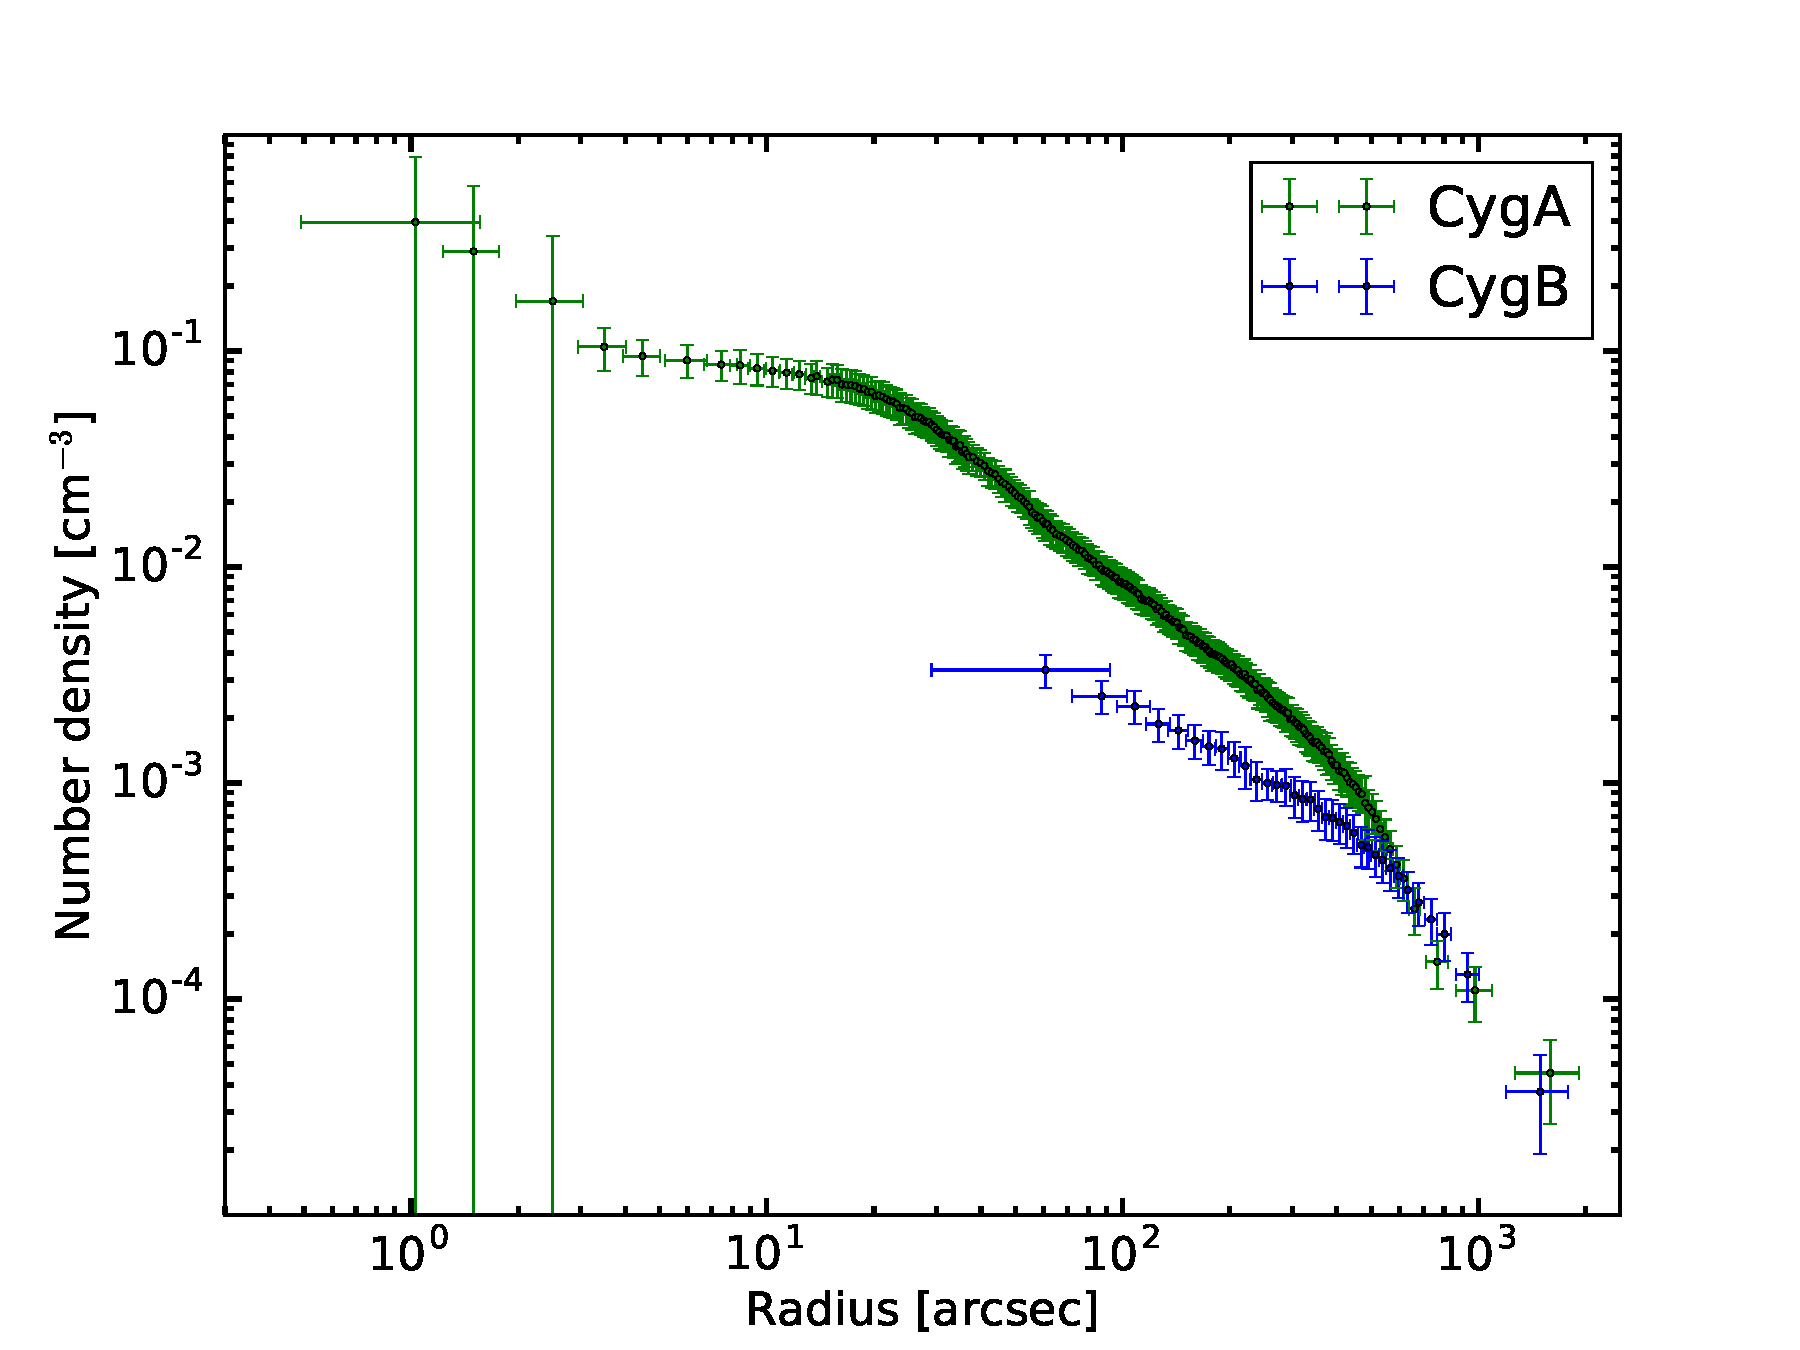
\includegraphics[width=1.3\textwidth]{ics/radial/raw_observed_clusters.pdf}}%
    \caption{Number density $n_e$ as a function of radius $r$ of the
    982~ksec \satellite{Chandra} observation \newline
    \citep[in prep]{2016MNRAS.123..456W} for CygA and CygB. Data courtesy of
    Martijn de Vries.}
    \label{fig:raw_data}
\end{figure}

TODO: double-check the numbers, and use both $n_e(r)$ and $T_g(r)$. This 
kills fluid approx which would be patched up with plasma magic ??
The number density and the average cluster temperature are plugged into the
equations presented in section~\ref{sec:clustergas}. Indeed, cooling trough 
line emission can be neglected as $T_g > 4 \cdot 10^7$~K 
% 8.5e10* (0.092/1e-3)**(-1) (6.85e7/1e8)**(1/2)
and eq.~\eqref{eq:coolingtime} is appropriate to approximate the cooling time.
Plugging in the temperature and central density of CygA yields $t_{\text{cool}} 
\approx 2 \times 10^{10}$ year, while this value increases to \mytilde $10^{12}$
around the virial radius. The virial radius of roughly $1345$~kpc is found using 
the models presented in section~\ref{sec:results-xray}.
% 1870*3.3e5*(6.85e7/1e8)**1.5*(0.092/1e-3)**(-1)
The longest equilibrium time eq.~\eqref{eq:tcoulomb} to achieve equipartition as
a result of Coulomb interactions gives $t_{\text{eq}}(p,e)$\mytilde $4\times 10^6$
in the core of CygA, increasing to \mytilde $4\times 10^9$ around the virial radius.
\citet{1988xrec.book.....S} gives a probable age of clusters of galaxies of $10^{10}$.
From this we can see that the age of the cluster and the cooling time are larger
than the timescale for Coulomb interactions and indeed the Maxwellian velocity 
distribution holds, thus satisfying requirement i) of the coronal limit assumption
and simultaneously satisfying requirement ii) of the fluid approximation. 
However, these numbers are significantly larger than the time steps taken in
the simulations. A full consideration of the plasma physics is required to 
justify the fluid approximation, which is beyond the scope of this thesis.


\subsection{Beta Model Fit}
\label{sec:results-xray}
The raw data presented in Figure~\ref{fig:raw_data} allows us to fit the 
beta-model (equation~\eqref{eq:betamodel} in section~\ref{sec:clustergas}) to
obtain the core radius, central density and the slope parameter $\beta$.
Two conversions take place prior to continuing our analysis. First, we convert
the electron number density to mass density by
\begin{align}
    \rho_{\text{gas}} (r) &= \mu m_p n_e(r) \label{eq:convert-neToRho} \\
    \mu &=  \frac{4}{5 x_H + 3} \quad ,
\end{align}
where $\mu$ is the mean molecular weight, $m_p$ is the proton mass in gram, and
$x_H$ is the hydrogen fraction, assuming $x_H = 0.76$. Second, we convert the 
radius from seconds of arc to kpc using equation~\eqref{eq:arcsec2kpc}.
Note that Cygnus~A has a redshift of $z=0.0562$ \citep{1997ApJ...488L..15O}, 
at which one conveniently finds that $1$" approximately corresponds to $1$ kpc.
As a rule of thumb, converting back and forth is as simple as swapping the unit
kpc for arcsecond. Slightly more precise, adopting a concordance cosmology with
$H_0=70$~km/s/Mpc, $\Omega_M=0.3$, $\Omega_\Lambda=0.7$, the conversion factor
found is $1$" \mytilde \, $1.091$.

If the merger is indeed $0.2-0.6$~Gyr prior to core passage \citep{2005AJ....130...47L},
the derived gas profile is a fairly good description of the relaxed sub clusters 
before the merger process has started. The values found here can thus be used
as initial conditions to set up the numerical simulations. We adopt two % three 
variations of the beta model. We show fit results where the slope is left as a 
free parameter, and assuming a fixed value of $\beta=2/3$. Initially, the 
numerical implementation of \code{Toycluster} \citep{2014MNRAS.438.1971D} assumed
this particular $\beta$-value, and for this reason we show the fit results for
the beta model where $\beta$ fixed to $2/3$. 
% Finally, we show fit results of the fixed beta model with an additional cut-off
% at the virial radius because the haloes are sampled with this slightly modified 
% beta model for numerical stability. 
The updated code that will be published by \citet[in prep]{2016MNRAS.000.000D} 
allows for any value of $\beta$. See section~\ref{sec:methods-toycluster} for
details of the numerical initial conditions code. The fit results are presented
in Table~\ref{tab:fits}. Figure~\ref{fig:free_betamodel_cygA_900ksec} shows a 
plot of the free $\beta$-model fit to the 982~ksec mass density profile of CygA, 
and Figure~\ref{fig:betamodel_cygA_900ksec} shows the fixed beta fit. Plots of 
fits to the CygB density are shown, respectively, in 
Figure~\ref{fig:free_betamodel_cygB_900ksec}, and 
Figure~\ref{fig:betamodel_cygB_900ksec}. 

\begin{table}
    \centering
    \caption{Fit parameters for our different physics models. We consider
    a beta-model with beta as a free parameter, and we fit the same model
    with $\beta$ fixed at $2/3$.} %  Finally, we show fit results of a cut-off
    % beta $2/3$ model because the clusters are numerically sampled with an
    % additional cut-off at the virial radius.
    \label{tab:fits}
    \begin{tabular}{llccl}
        \hline
        Model & Quantity & CygA & CygB & Unit \\
        \hline
        % because numerics
        % from fit to Chandra data
        free beta & $\beta$ & $0.538 \pm 0.007$ & $0.790 \pm0.072$ \\
                  & $n_{e,0}$  & ($9.162 \pm 0.417) \times 10^{-2}$ & $(2.28 \pm 0.15) \times 10^{-3}$ & cm$^{-3}$ \\
                           & $r_c$ & $ 26.02 \pm 1.235 $  & $ 305.8 \pm 36.16 $ & kpc \\
                   & $\chi_{\text{min}}^2$ & 224.2 & 14.40 \\
                   & dof & 222 & 32 \\
                   & p-value & 0.44522 & 0.99684 \\
        beta & $\beta$ (fixed) & 2/3 & 2/3 \\
             & $n_{e,0}$  & $(5.939 \pm 0.268) \times 10^{-2} $ & $(2.54 \pm 0.15) \times 10^{-3}$ & cm$^{-3}$ \\
                   & $r_c$ & $48.39 \pm 1.498$  & $238.6 \pm 11.06$ & kpc \\
                   & $\chi_{\text{min}}^2$ & 462.0 & 15.71 \\
                   & dof & 223 & 33 \\
                   & p-value & 0.00000 & 0.99529 \\
        % cut-off beta & $\beta$ (fixed) & 2/3 & 2/3 \\
        %              & $n_{e,0}$  & $(5.905 \pm 0.267) \times 10^{-2}$ & $(2.34 \pm 0.11) \times 10^{-3}$  & cm$^{-3}$ \\
        %                    & $r_c$ & $ 48.64 \pm 1.520$ & $264.6 \pm 11.51$ & kpc \\
        %                    & $r_{\text{cut}}$ & $ 1754.97 \pm 717.37 $  & $ 1313.83 \pm 124.34 $ & kpc \\
        %            & $\chi_{\text{min}}^2$ & 460.4 & 9.323\\
        %            & dof & 222 & 32 \\
        %            & p-value & $0.00000$ & $0.99997$ \\
        \hline
    \end{tabular}
\end{table}


\begin{figure}[p]
    % \includegraphics[width=0.9\textwidth]{ics/density_betamodel_fit_cygA_800ksec.png}
    % \caption{Cygnus~A $\beta (2/3)$ model fit to the 799.5~ksec
    % \satellite{Chandra} observation
    % \citep[in prep]{2016MNRAS.123..456W}. The dashed
    % vertical line indicates the core radius $r_c$.}
    % \label{fig:betamodel_cygA_800ksec}
    \centering
    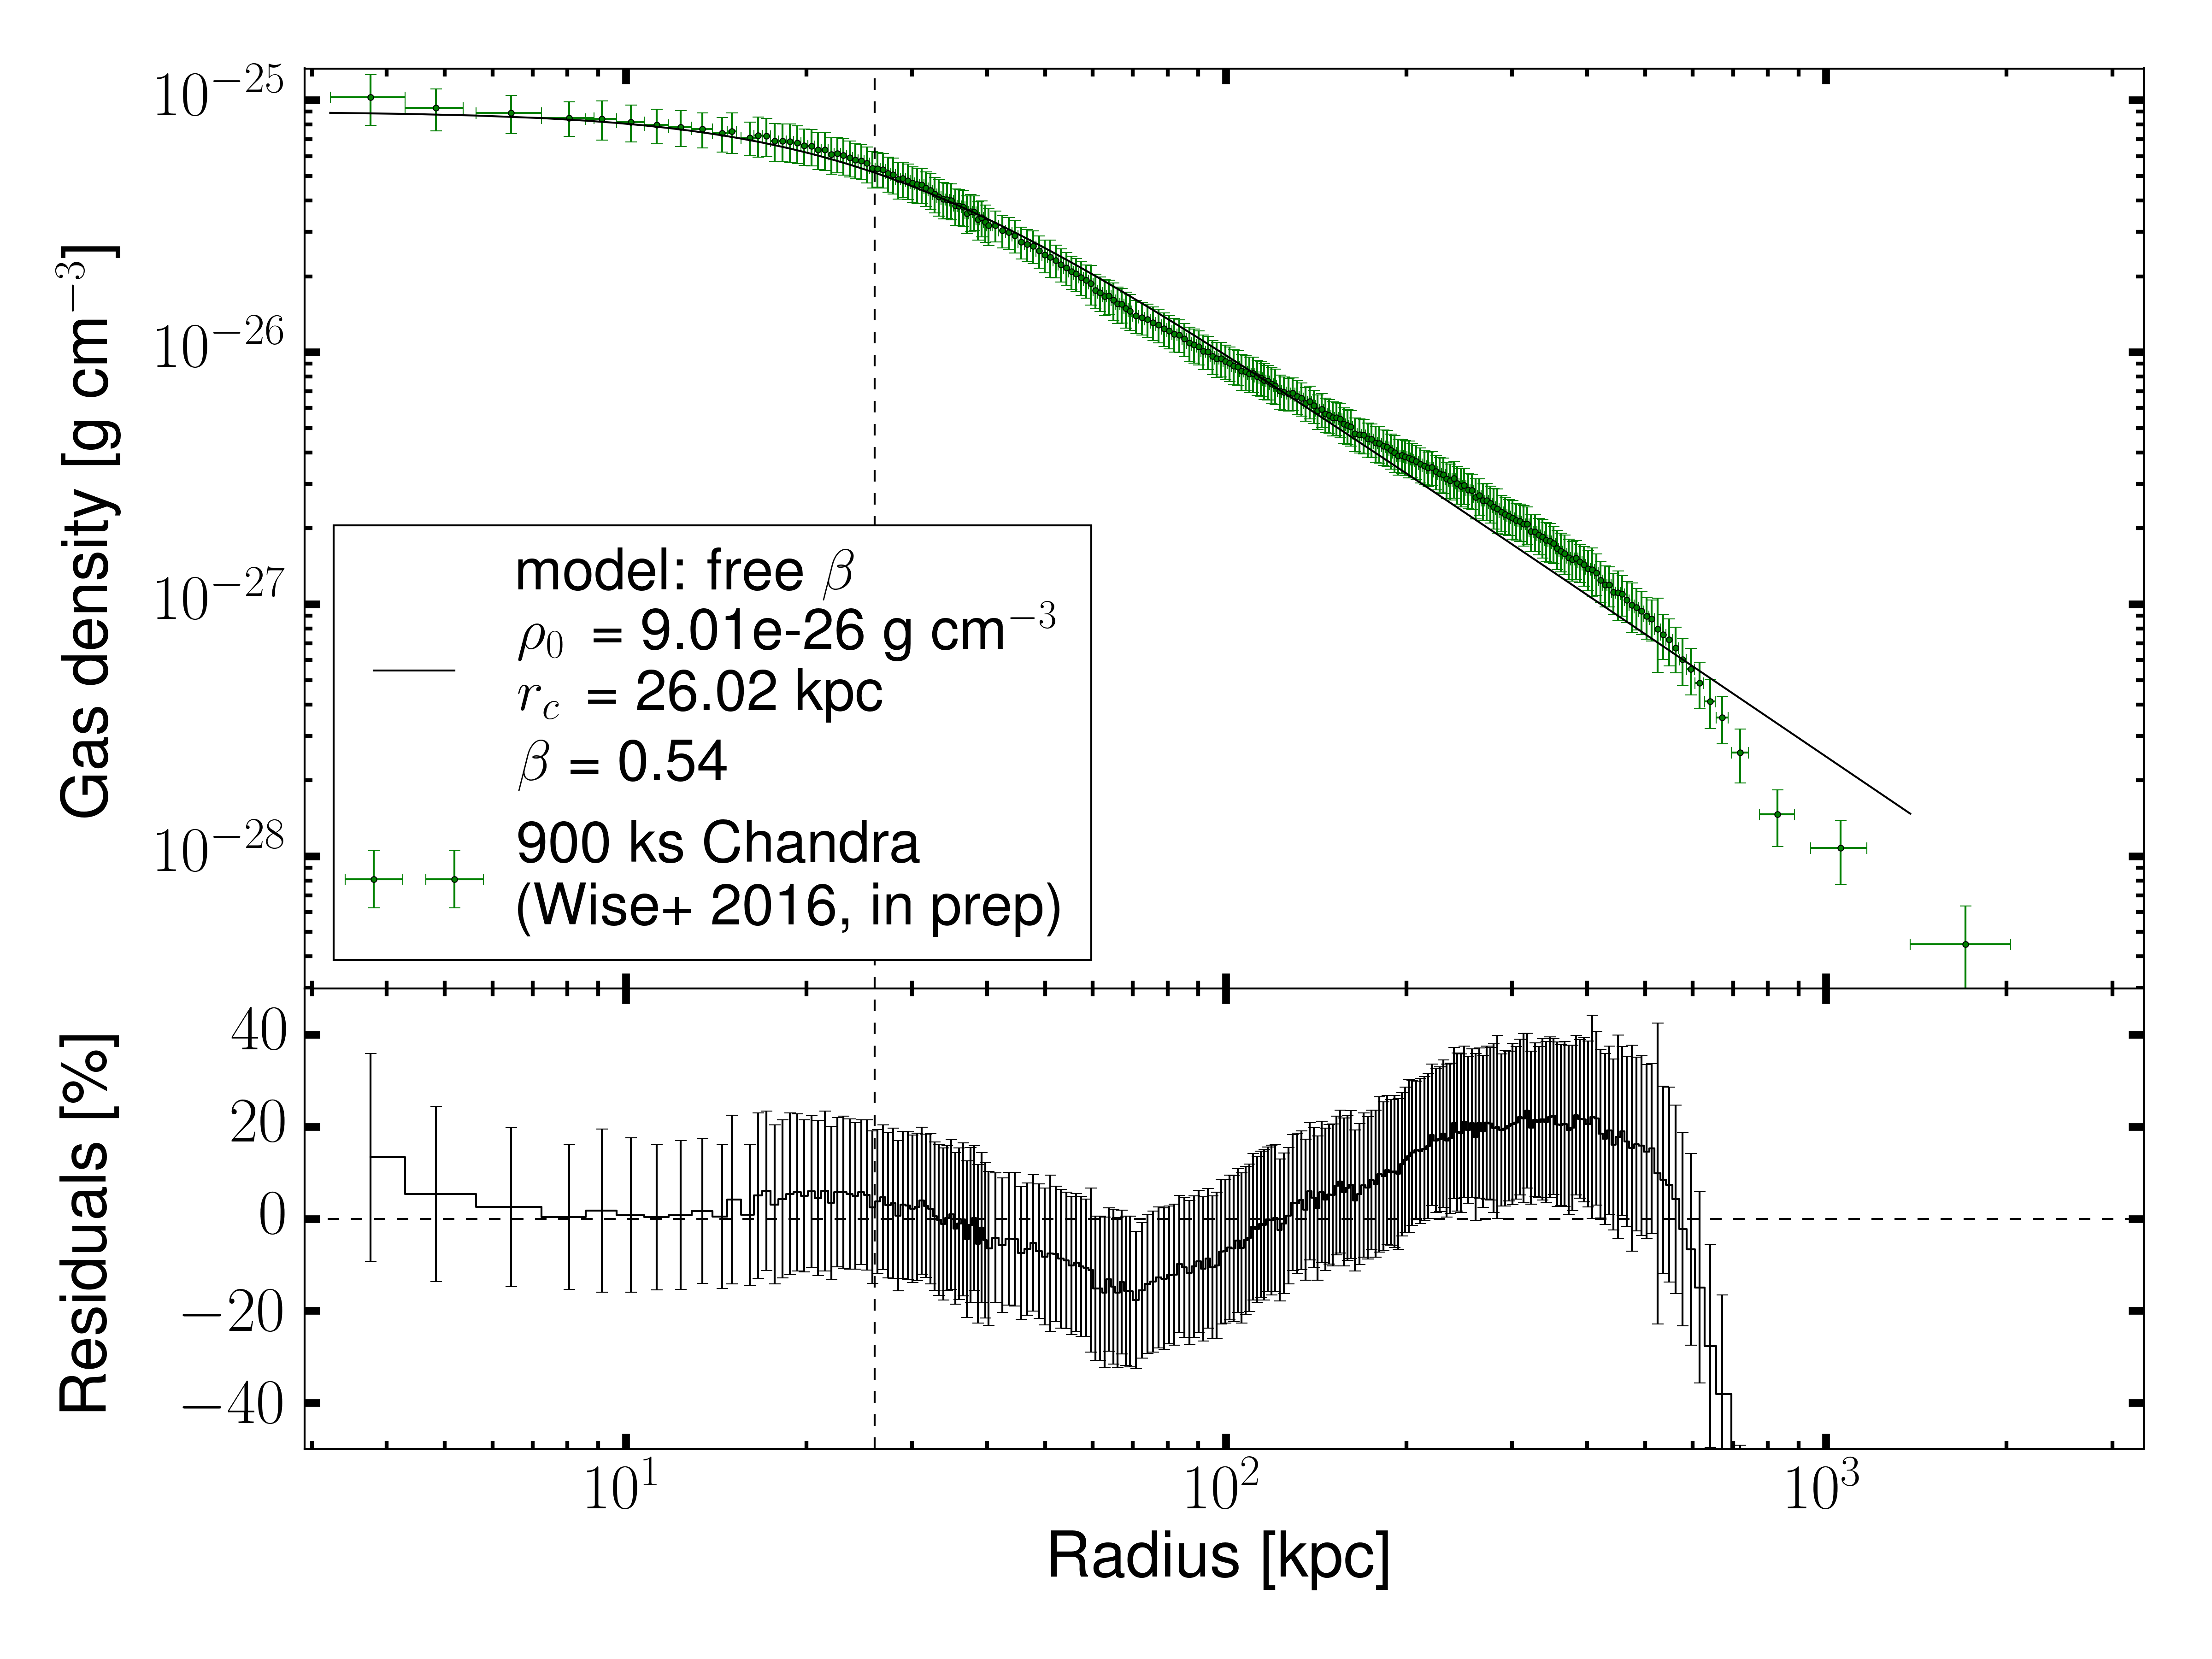
\includegraphics[width=0.9\textwidth]{ics/radial/density_free_betamodel_fit_cygA_900ksec.png}
    \caption{Cygnus~A $\beta$ model fit to the \mytilde982~ksec
    \satellite{Chandra} observation \citep[in prep]{2016MNRAS.123..456W}. \newline The dashed
    vertical line indicates the core radius $r_c$. Here $\beta$ is as a free parameter.}
    \label{fig:free_betamodel_cygA_900ksec}
    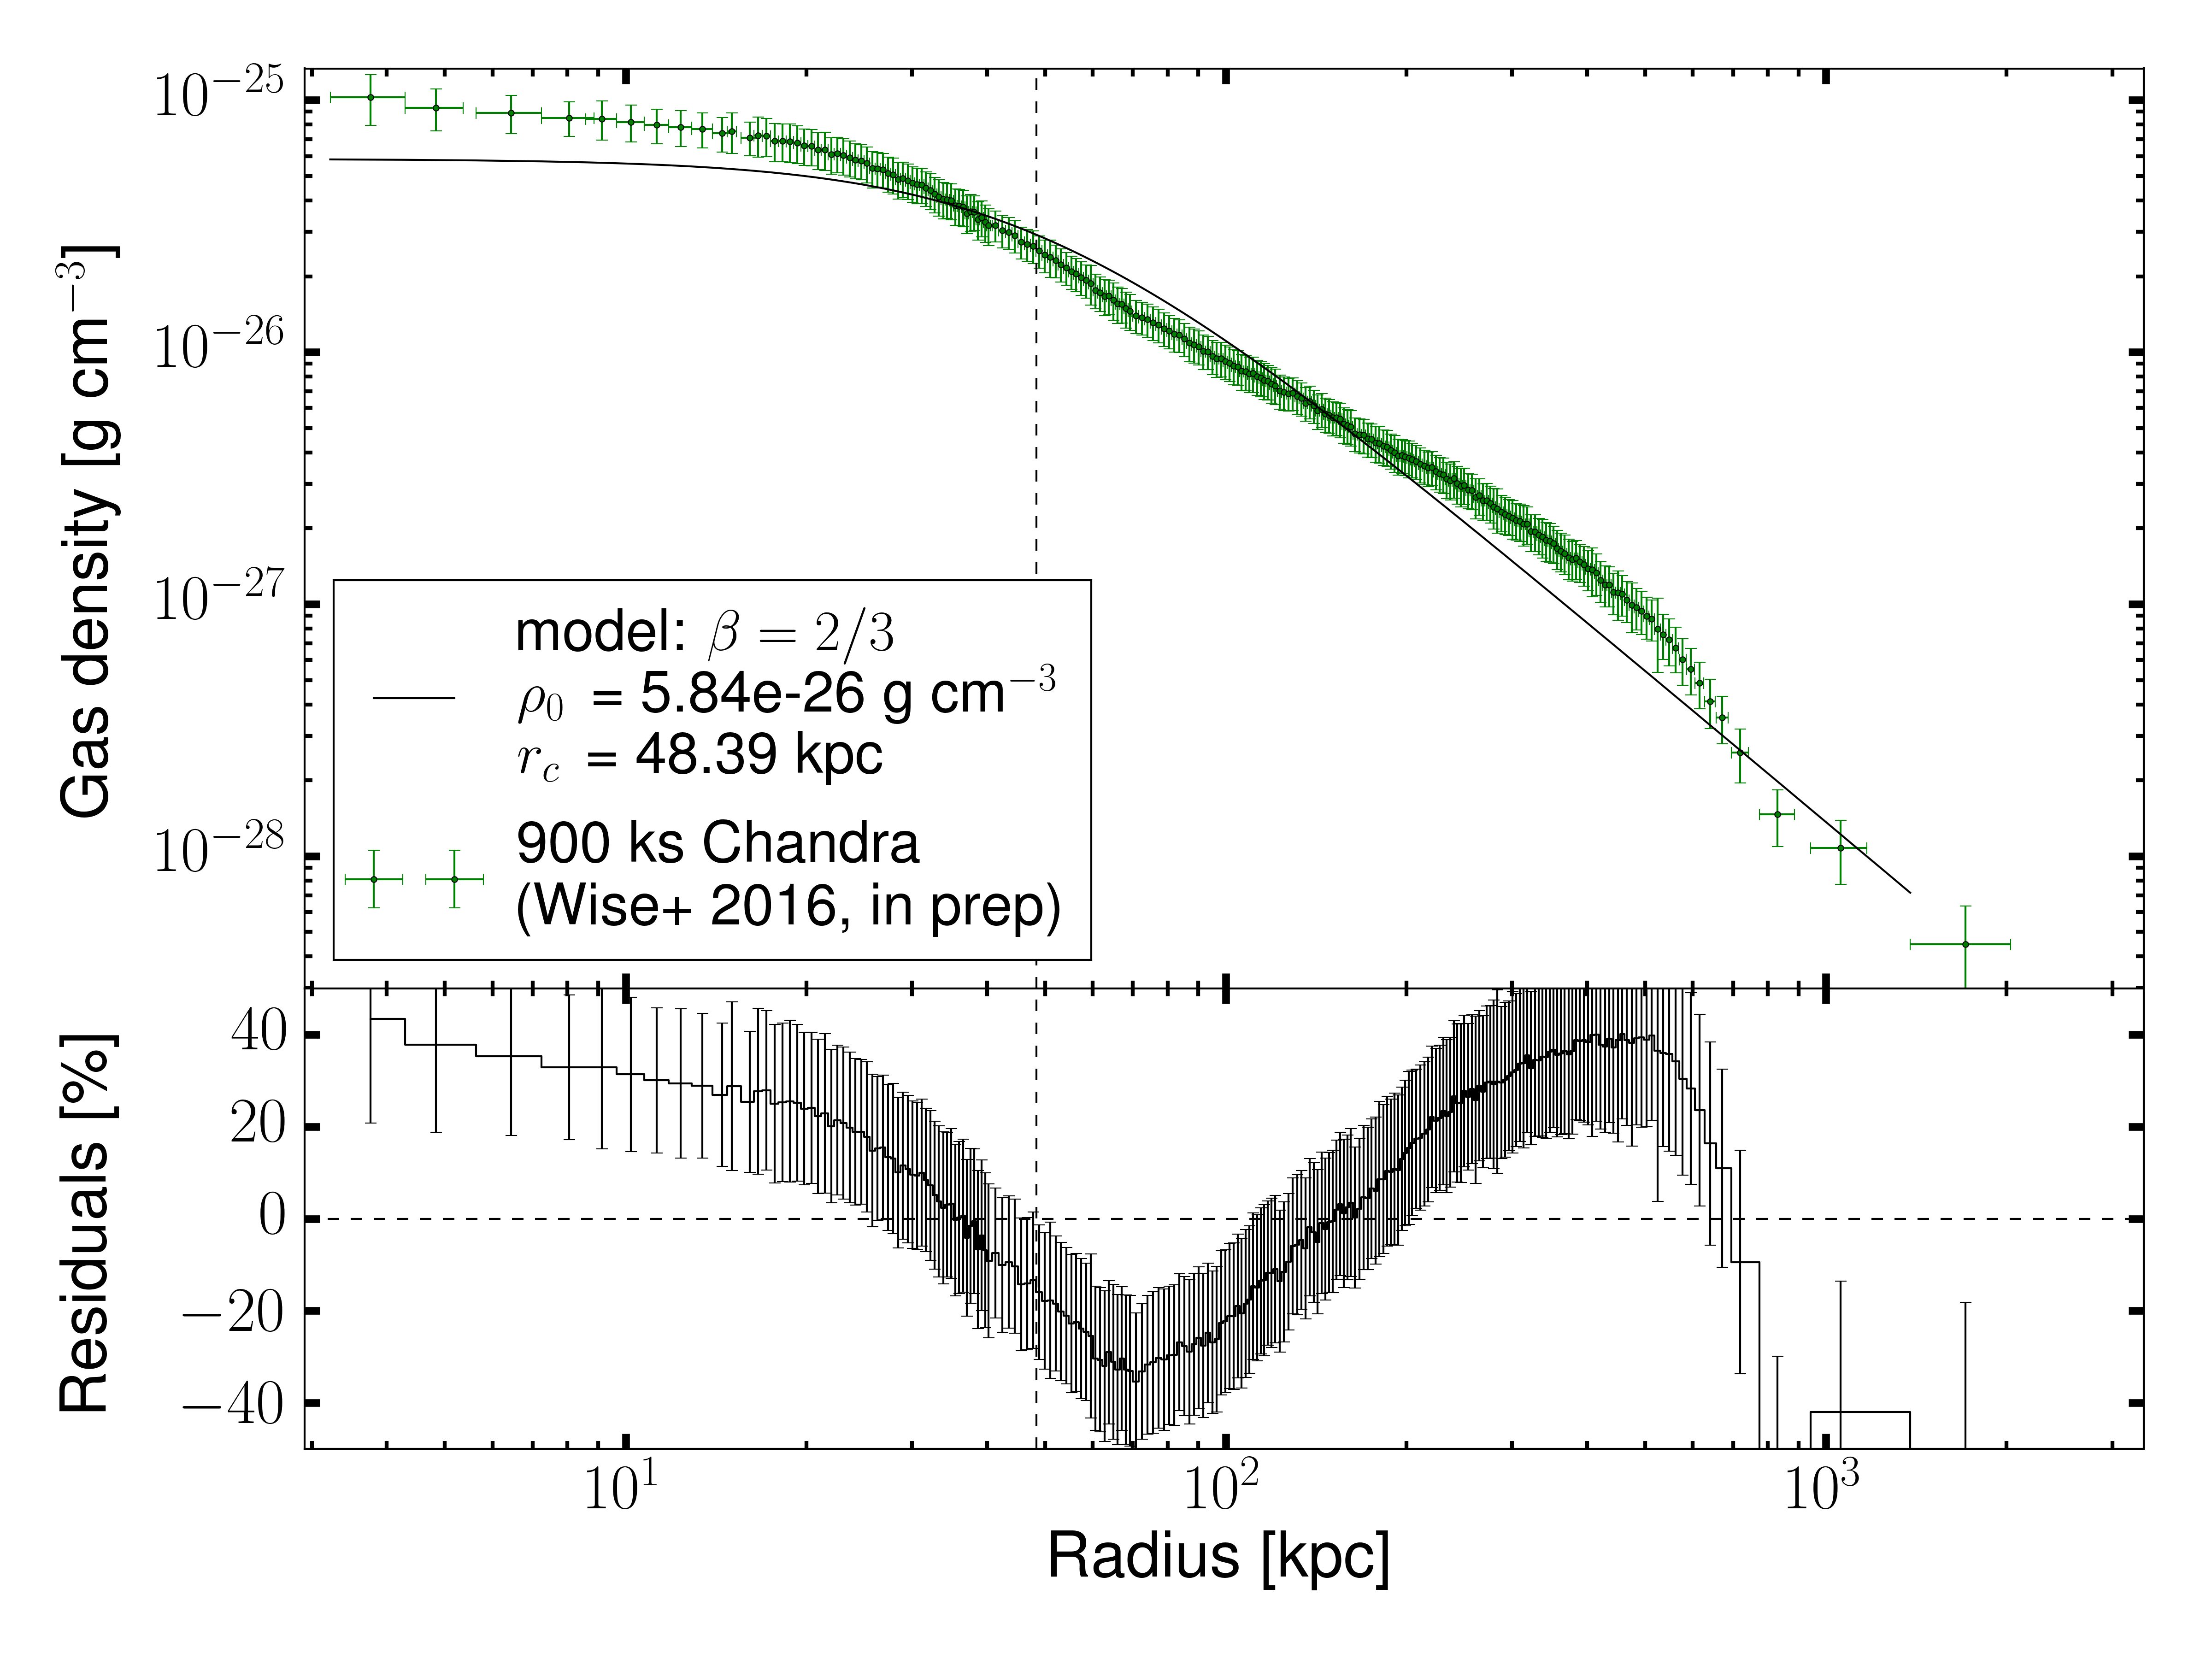
\includegraphics[width=0.9\textwidth]{ics/radial/density_betamodel_fit_cygA_900ksec.png}
    \caption{Cygnus~A $\beta=2/3$ model fit to the \mytilde982~ksec
    \satellite{Chandra} observation \citep[in prep]{2016MNRAS.123..456W}.
    \newline The dashed vertical line indicates the core radius $r_c$.}
    \label{fig:betamodel_cygA_900ksec}
\end{figure}
\begin{figure}[p]
    % \includegraphics[width=0.9\textwidth]{ics/density_betamodel_fit_cygB_800ksec.png}
    % \caption{Cygnus~B $\beta=2/3$ model fit to the 799.5~ksec
    % \satellite{Chandra} observation
    % \citep[in prep]{2016MNRAS.123..456W}. The dashed
    % vertical line indicates the core radius $r_c$.}
    % \label{fig:betamodel_cygB_800ksec}
    \centering
    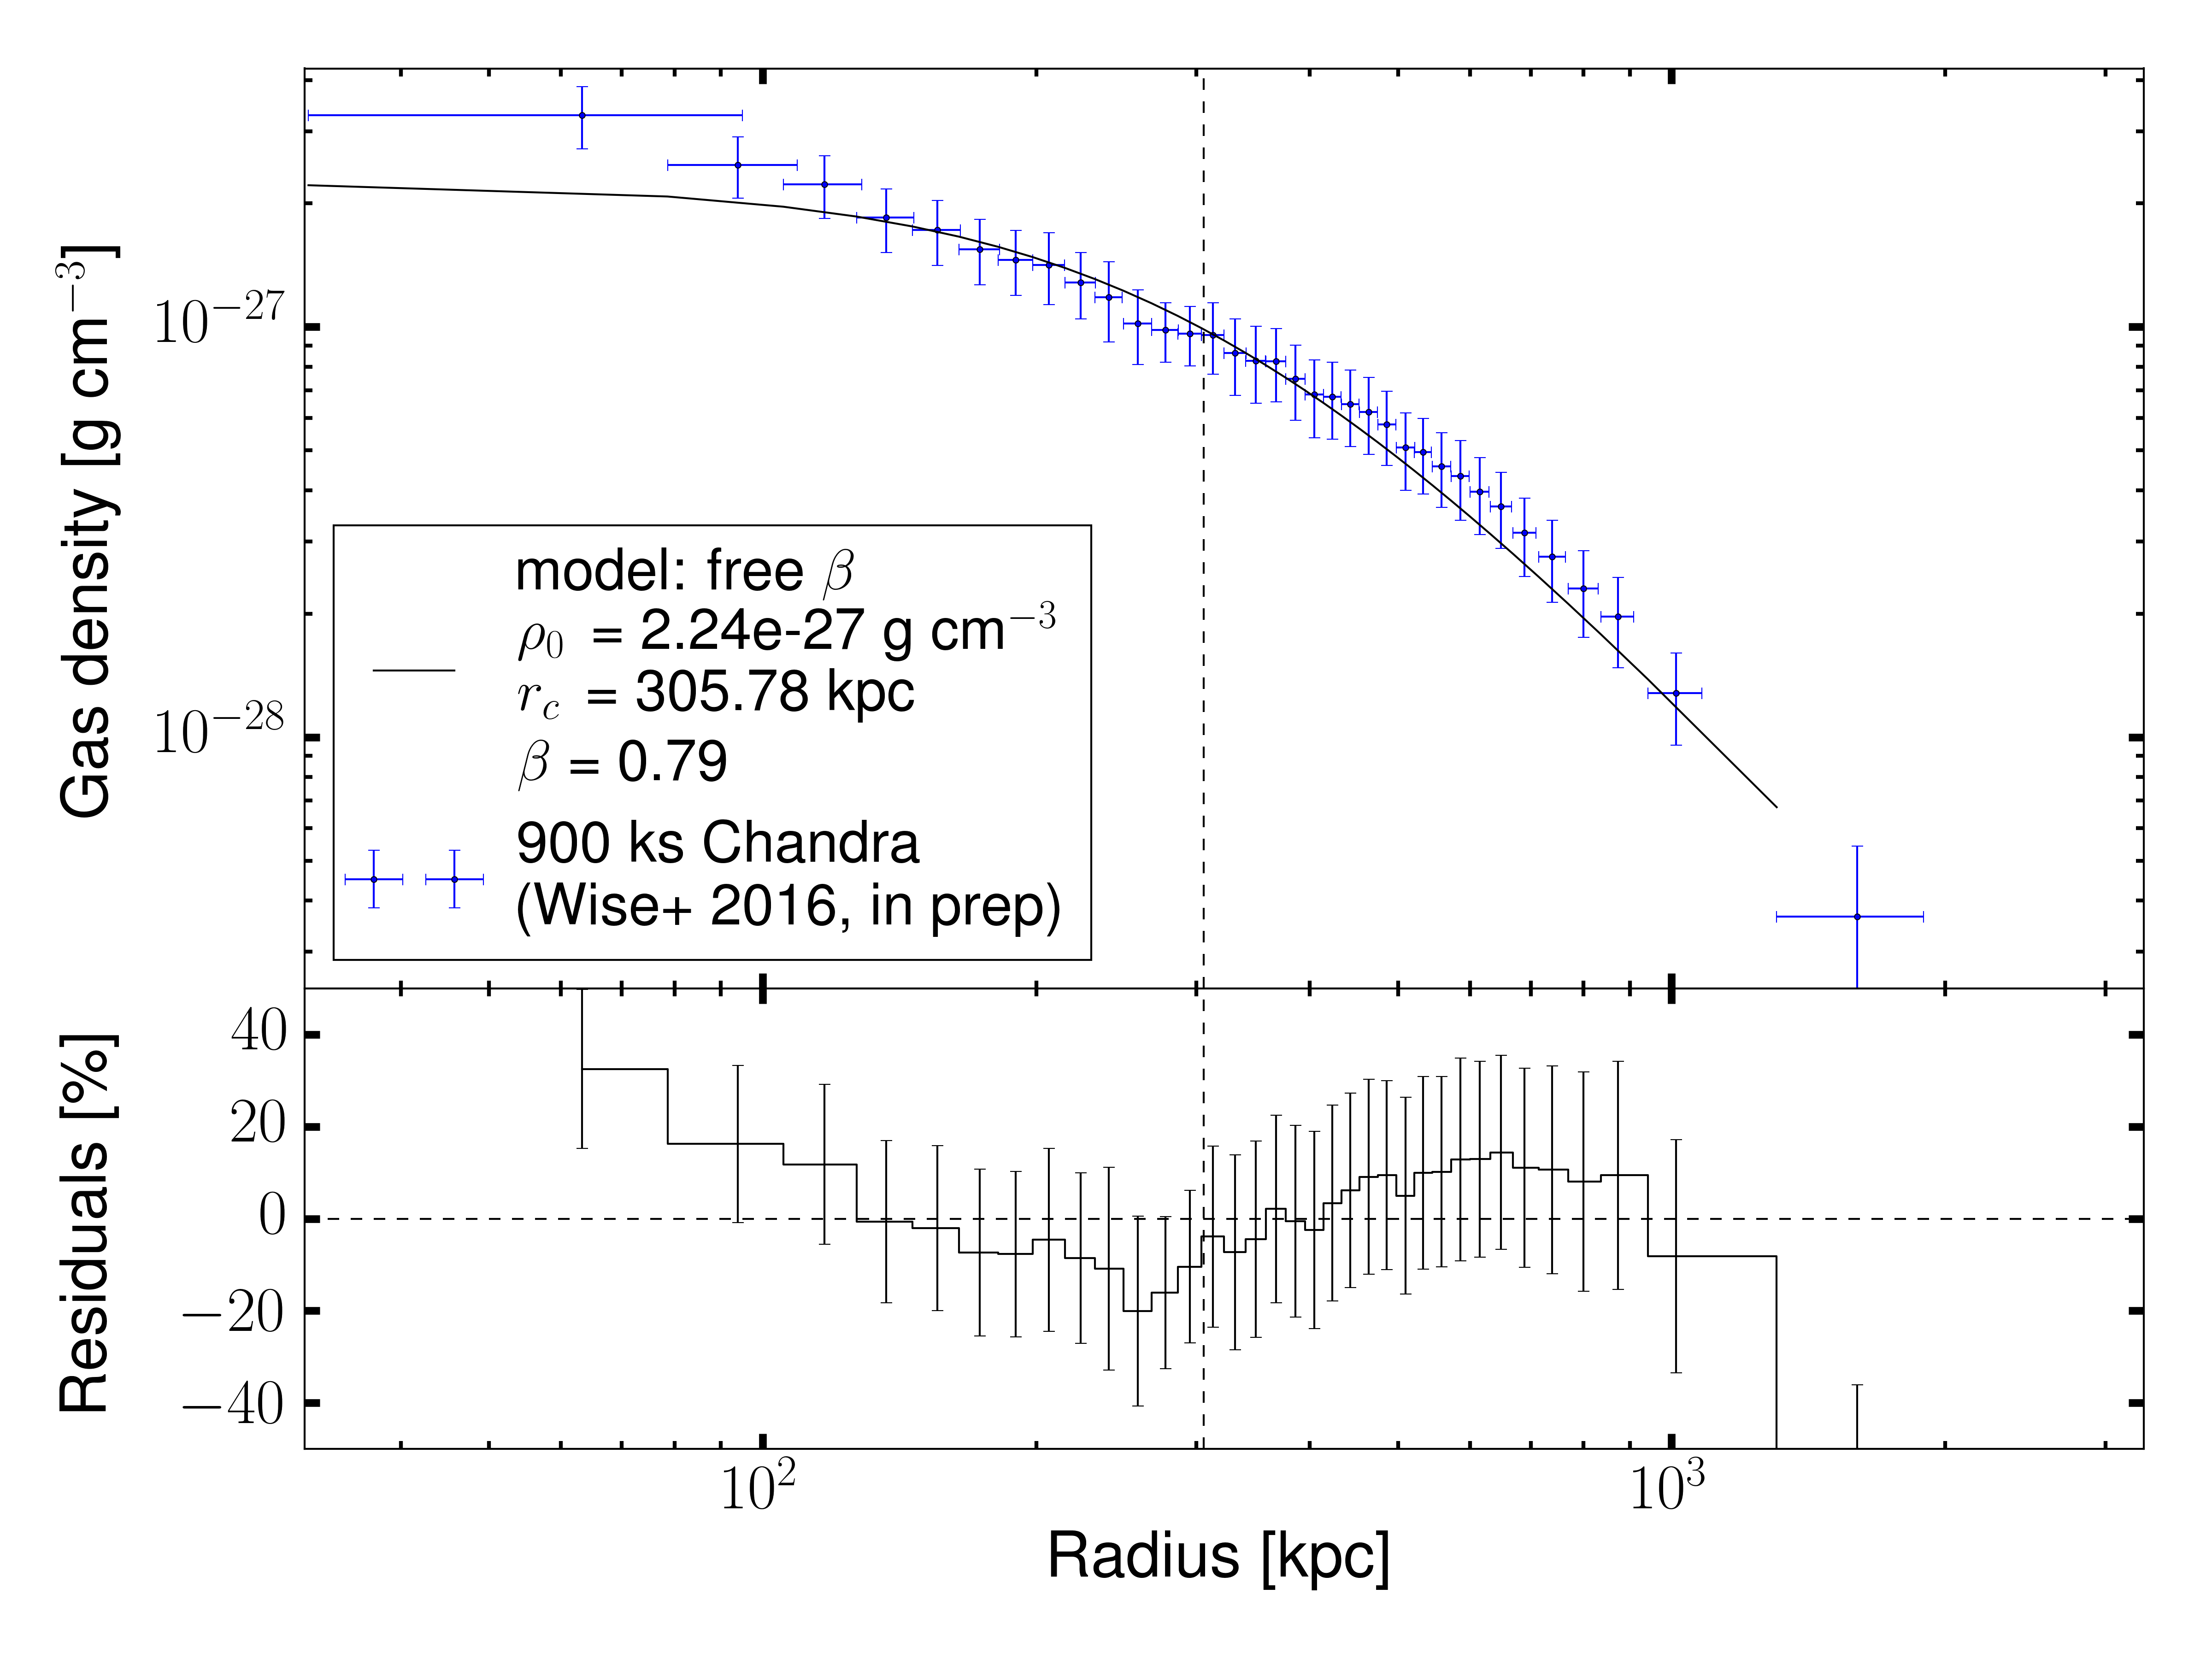
\includegraphics[width=0.9\textwidth]{ics/radial/density_free_betamodel_fit_cygB_900ksec.png}
    \caption{Cygnus~B $\beta$ model fit to the \mytilde900~ksec
    \satellite{Chandra} observation \citep[in prep]{2016MNRAS.123..456W}. \newline The dashed
    vertical line indicates the core radius $r_c$. Here $\beta$ is a free parameter.}
    \label{fig:free_betamodel_cygB_900ksec}
    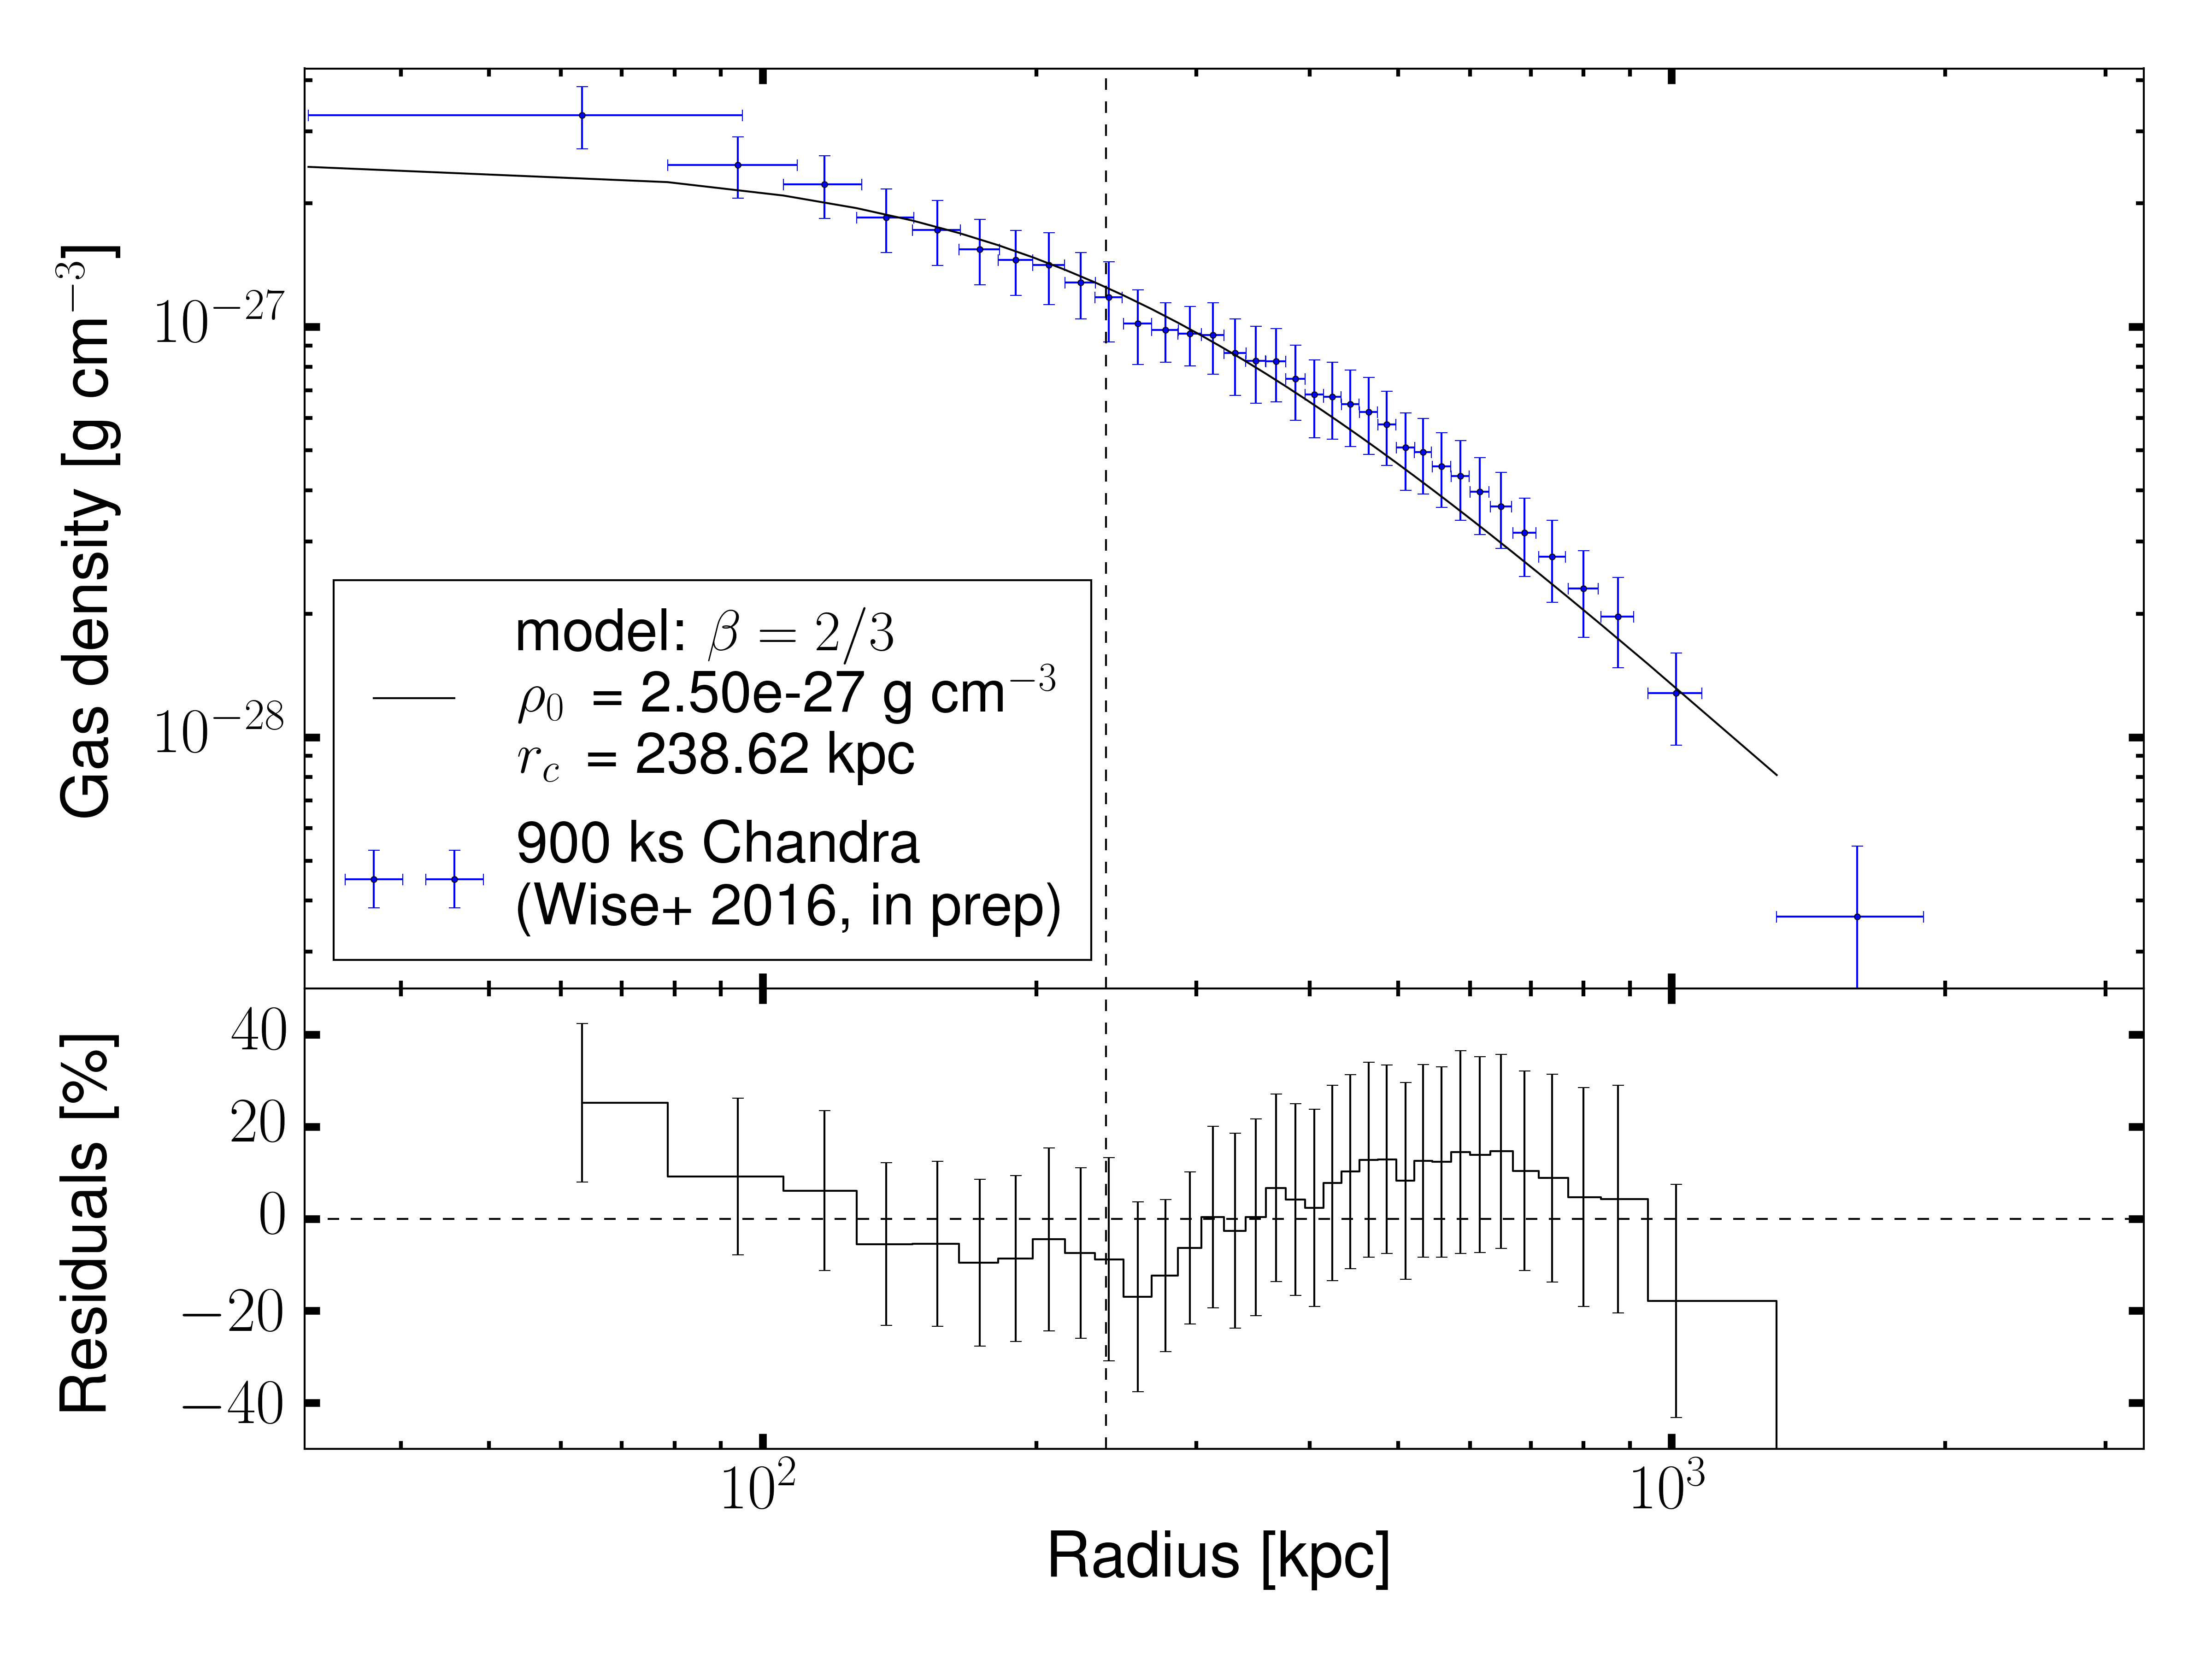
\includegraphics[width=0.9\textwidth]{ics/radial/density_betamodel_fit_cygB_900ksec.png}
    \caption{Cygnus~B $\beta=2/3$ model fit to the \mytilde900~ksec
    \satellite{Chandra} observation \citep[in prep]{2016MNRAS.123..456W}. \newline The dashed
    vertical line indicates the core radius $r_c$.}
    \label{fig:betamodel_cygB_900ksec}
\end{figure}


\newpage
\subsection{From Gas Density to Total Gravitating Mass}
\label{sec:gas-to-dm}
The initial conditions code \code{Toycluster} starts from the total gravitating
mass $M_{200}$ within the virial radius $r_{200}$. This works perfectly when the 
cluster mass including the contribution of the dark matter halo is obtained 
trough a weak lensing studies of the cluster of galaxies of interest. The 
baryonic cluster properties can then be calculated under the assumption of 
a fixed baryon fraction at the virial radius $b_f(r_{200})=0.17$. To the best
of our knowledge, however, no results of a weak lensing study of the Cygnus 
cluster have been published as of August 2016. We do have, on the other hand, 
excellent constrains on the gas profile from the X-ray observations, which allows
us to do the calculation the other way around. We infer the dark matter properties
from the measured gas profiles as the beta model is fully constrained from the
observed core radius, central density and $\beta$. The method presented in this
section therefore predicts the properties of the dark matter haloes. It is known
that dark matter in general follows the NFW-profile, which depends on the scale
radius $r_s = r_{200}/c_{\text{NFW}}$ where $c_{\text{NFW}}$ is the concentration
parameter. This quantity is also given by \citet{2008MNRAS.390L..64D} as a 
function of $M_{200}$.

\begin{align}
    c_{\text{NFW}} &= 5.74 \left( \frac{M_{200}}{2 \times 10^{12} h^{-1} M_\odot} \right)^{-0.097}
\end{align}

\code{Toycluster} uses the Hernquist profile rather than the NFW-profile, both
of which are equal within the scale radius $r_s$ when the central density of 
both profiles is the same and the Hernquist scale length $a$ is calculated as a
function of the concentration parameter using equation~\eqref{eq:a_hernquist}.

Assuming a fixed baryon fraction at the virial radius

\begin{align}
    b_f(r_{200}) &= \frac{M\text{gas}(r_{200})}{M\text{gas}(r_{200}) + M\text{dm}(r_{200})} = 0.17 \\
                 &\Rightarrow M\text{dm}(r_{200}) = M\text{gas}(r_{200})\left(\frac{1}{b_f(r_{200})} - 1 \right) \quad , \\
\end{align}
\noindent allows us to calculate $M_{200}$ only if we know $r_{200}$. The gas 
mass $M_{\text{gas}(r_{200})}$ follows by integrating the density profile 
(beta-model) over the volume under the assumption of spherical symmetry and
plugging in the virial radius.

The concentration parameter $c_{\text{NFW}}$ depends only on the total 
gravitating mass $M_{200}$, which in turn depends on the virial radius.
Furthermore, to obtain the Hernquist scale length we need to know both
the concentration parameter and the scale radius $r_s$, which also depends 
on the virial radius. If the Hernquist scale length is known, we can then 
obtain the total dark matter mass $M_{\text{DM}}$ by dividing the value of 
$M_{\text{DM}(r_{200})}$ matter mass profile at $r_{200}$. This fully constrains
the dark matter profile. If only we knew the value of $r_{200}$ all of the
required quantities could easily be computed. Now, remembering the definition 
of the virial radius sets the following condition.

\begin{align}
    \overline{\rho}(<r_{200}>) &= 200 \rho_{\text{crit}} \\
    &\Rightarrow \left(\frac{M_{200}}{\frac{4}{3} \pi r_{200}^3} \right) \cdot
    \left( \frac{1}{\rho_{\text{crit}}} \right) = 200 \label{eq:hack}
\end{align}

This allows us to implicitly solve the problem by trial-and-error of virial 
radius values such that both the baryon fraction at the tried virial radius 
equals 17 per cent and Equation~\eqref{eq:hack} is satisfied. This is implemented
numerically by using the bisection method, which results in the values presented
in Table~\ref{tab:parameters}. Note that the mass is obtained by integrating the
beta-model over the volume, which results in the Gaussian Hypergeometrical 
function, equation~\eqref{eq:hypergeometrical}, in the free-beta case. The 
numerical implementation to obtain the mass we use is provided by \code{SciPy}
for \code{Python} scripts, and by the GNU Scientific Library for the 
\code{c}-language. However, due to domain restrictions in the latter, a set of 
transformations presented in appendix~\ref{sec:hypertrafo} is required to stay
within the valid domain range and allows us to use these implementations. As a
final remark, the quantities inferred from the observations are provided with 
the $1 \sigma$ uncertainties. The uncertainties of the inferred dark matter are 
dominated by (unknown) systematic error margins. Simply propagating the 
statistical error would present the results with a higher certainty than we can
actually justify, which is why no such estimates are provided in the table.


\begin{table}
    \centering
    \caption{Initial Conditions for the CygA and CygB sub clusters.
             The central density and core radius are obtained from a
             beta-model fit to the \satellite{Chandra} data, both for
             beta as a free parameter, and with beta fixed at $2/3$. 
             All other quantities are obtained using the \citep{1990ApJ...356..359H}
             dark matter profile under the assumption that 
             $b_f =0.17$ within $r_{200}$. Only for the observed quantities 
             the 1 $\sigma$ (statistical) uncertainty is quoted.}
    \label{tab:parameters}
    \begin{tabular}{llccl}
        \hline
        Model & Quantity & CygA & CygB & Unit \\
        \hline
        % from fit to Chandra data
        free beta & $\beta$ & $0.538 \pm 0.007$ & $0.790\pm0.072$ & \\
        & $n_{e,0}$ & $(9.162 \pm 0.417) \cdot 10^{-2}$ & $(2.28 \pm 0.15) \cdot 10^{-3}$ & cm$^{-3}$ \\
        & $\rho_{0, \text{gas}}$ & $(9.014 \pm 0.410) \cdot 10^{-26}$ & $(2.243\pm0.145) \cdot 10^{-27}$ & g cm$^{-3}$ \\ 
        & $r_c$ & $26.016 \pm 1.236$ & $305.78 \pm 36.16$ & kpc \\
        % % From Hernquist profile plus assumption bf(r200) = 0.17
        % & $r_{200}$ & $1347.52^{47.08}_{-49.62}$ & $923.13^{+58.30}_{-60.86}$ & kpc \\
        % & $M_{\text{gas200}}$ & $4.991^{+0.542}_{-0.531} \cdot 10^{13}$ & $1.605^{+0.324}_{-0.297} \cdot 10^{13}$  & M\Sun  \\
        % & $M_{\text{dm200}}$ & $2.437^{+0.265}_{-0.259} \cdot 10^{14}$ & $7.835^{+1.580}_{-1.450} \cdot 10^{13}$ & M\Sun \\
        % & $M_{200}$ & $2.936^{+0.320}_{-0.313} \cdot 10^{14}$ & $9.439^{+1.904}_{-1.747} \cdot 10^{13}$ & M\Sun \\
        % & $c_{\text{NFW}}$ & $3.662^{+0.040}_{-0.036}$ & $4.089^{+0.082}_{-0.072}$ & \\
        % & $r_s$ & $367.94^{+16.68}_{-17.40}$ & $225.79^{+18.57}_{-19.03}$ & kpc \\
        % & $a_{\text{Hernquist}}$ & $557.22^{+23.48}_{-24.57}$ & $353.45^{+27.06}_{-27.89}$ & kpc \\
        % & $M_{\text{DM}}$ & $4.869^{+0.550}_{-0.538} \cdot 10^{14}$ & $1.498^{+0.315}_{-0.287} \cdot 10^{14}$ & M\Sun  \\
        % From Hernquist profile plus assumption bf(r200) = 0.17
        & $r_{200}$ & $1347.52$ & $923.13$ & kpc \\
        & $M_{\text{gas200}}$ & $4.991 \cdot 10^{13}$ & $1.605 \cdot 10^{13}$  & M\Sun  \\
        & $M_{\text{dm200}}$ & $2.437 \cdot 10^{14}$ & $7.835 \cdot 10^{13}$ & M\Sun \\
        & $M_{200}$ & $2.936 \cdot 10^{14}$ & $9.439 \cdot 10^{13}$ & M\Sun \\
        & $c_{\text{NFW}}$ & $3.662$ & $4.089$ & \\
        & $r_s$ & $367.94$ & $225.79$ & kpc \\
        & $a_{\text{Hernquist}}$ & $557.22$ & $353.45$ & kpc \\
        & $M_{\text{DM}}$ & $4.869 \cdot 10^{14}$ & $1.498 \cdot 10^{14}$ & M\Sun  \\
        % because numerics
        %
        beta & $\beta$ (fixed) & $2/3$ & $2/3$ \\
        % from fit to Chandra data
        & $n_{e,0}$ & $(5.939 \pm 0.268) \cdot 10^{-2}$ & $(2.54 \pm 0.15) \cdot 10^{-3}$ & cm$^{-3}$  \\
        & $\rho_{0, \text{gas}}$ & $(5.843 \pm 0.263) \cdot 10^{-26}$ & $(2.499 \pm 0.14) \cdot 10^{-27}$ & g cm$^{-3}$ \\
        & $r_c$ & $48.389 \pm 1.498$ & $238.62 \pm 11.06$ & kpc \\
        % From Hernquist profile plus assumption bf(r200) = 0.17
        % & $r_{200}$ & $1076.9^{+58.993}_{-58.002}$ & $924.23^{+78.29}_{-76.18}$ & kpc \\
        % & $M_{\text{gas200}}$ & $2.547^{+0.442}_{-0.390} \cdot 10^{13}$ & $1.610^{+0.445}_{-0.366} \cdot 10^{13}$ & M\Sun  \\
        % & $M_{\text{dm200}}$ & $1.244^{+0.216}_{-0.190} \cdot 10^{14}$ & $7.862^{+2.172}_{-1.788} \cdot 10^{13}$ & M\Sun \\
        % & $M_{200}$ & $1.498^{+0.260}_{-0.229} \cdot 10^{14}$ & $9.473^{+2.617}_{-2.155} \cdot 10^{13}$ & M\Sun \\
        % & $c_{\text{NFW}}$ & $3.909^{+0.063}_{-0.060}$ & $4.087^{+0.104}_{-0.096}$ & \\
        % & $r_s$ & $275.47^{+19.64}_{-19.00}$ & $226.13^{+25.03}_{-23.77}$ & kpc \\
        % & $a_{\text{Hernquist}}$ & $425.50^{+28.208}_{-27.439}$ & $353.95^{+36.43}_{-34.86}$ & kpc \\
        % & $M_{\text{DM}}$ & $2.421^{+0.438}_{-0.384} \cdot 10^{14}$ & $1.504^{+0.4333}_{-0.3533} \cdot 10^{14}$ & M\Sun  \\
        & $r_{200}$ & $1076.9$ & $924.23$ & kpc \\
        & $M_{\text{gas200}}$ & $2.547 \cdot 10^{13}$ & $1.610 \cdot 10^{13}$ & M\Sun  \\
        & $M_{\text{dm200}}$ & $1.244 \cdot 10^{14}$ & $7.862 \cdot 10^{13}$ & M\Sun \\
        & $M_{200}$ & $1.498 \cdot 10^{14}$ & $9.473 \cdot 10^{13}$ & M\Sun \\
        & $c_{\text{NFW}}$ & $3.909$ & $4.087$ & \\
        & $r_s$ & $275.47$ & $226.13$ & kpc \\
        & $a_{\text{Hernquist}}$ & $425.50$ & $353.95$ & kpc \\
        & $M_{\text{DM}}$ & $2.421 \cdot 10^{14}$ & $1.504 \cdot 10^{14}$ & M\Sun  \\
        \hline
    \end{tabular}
\end{table}

%\begin{figure}
%    \centering
%    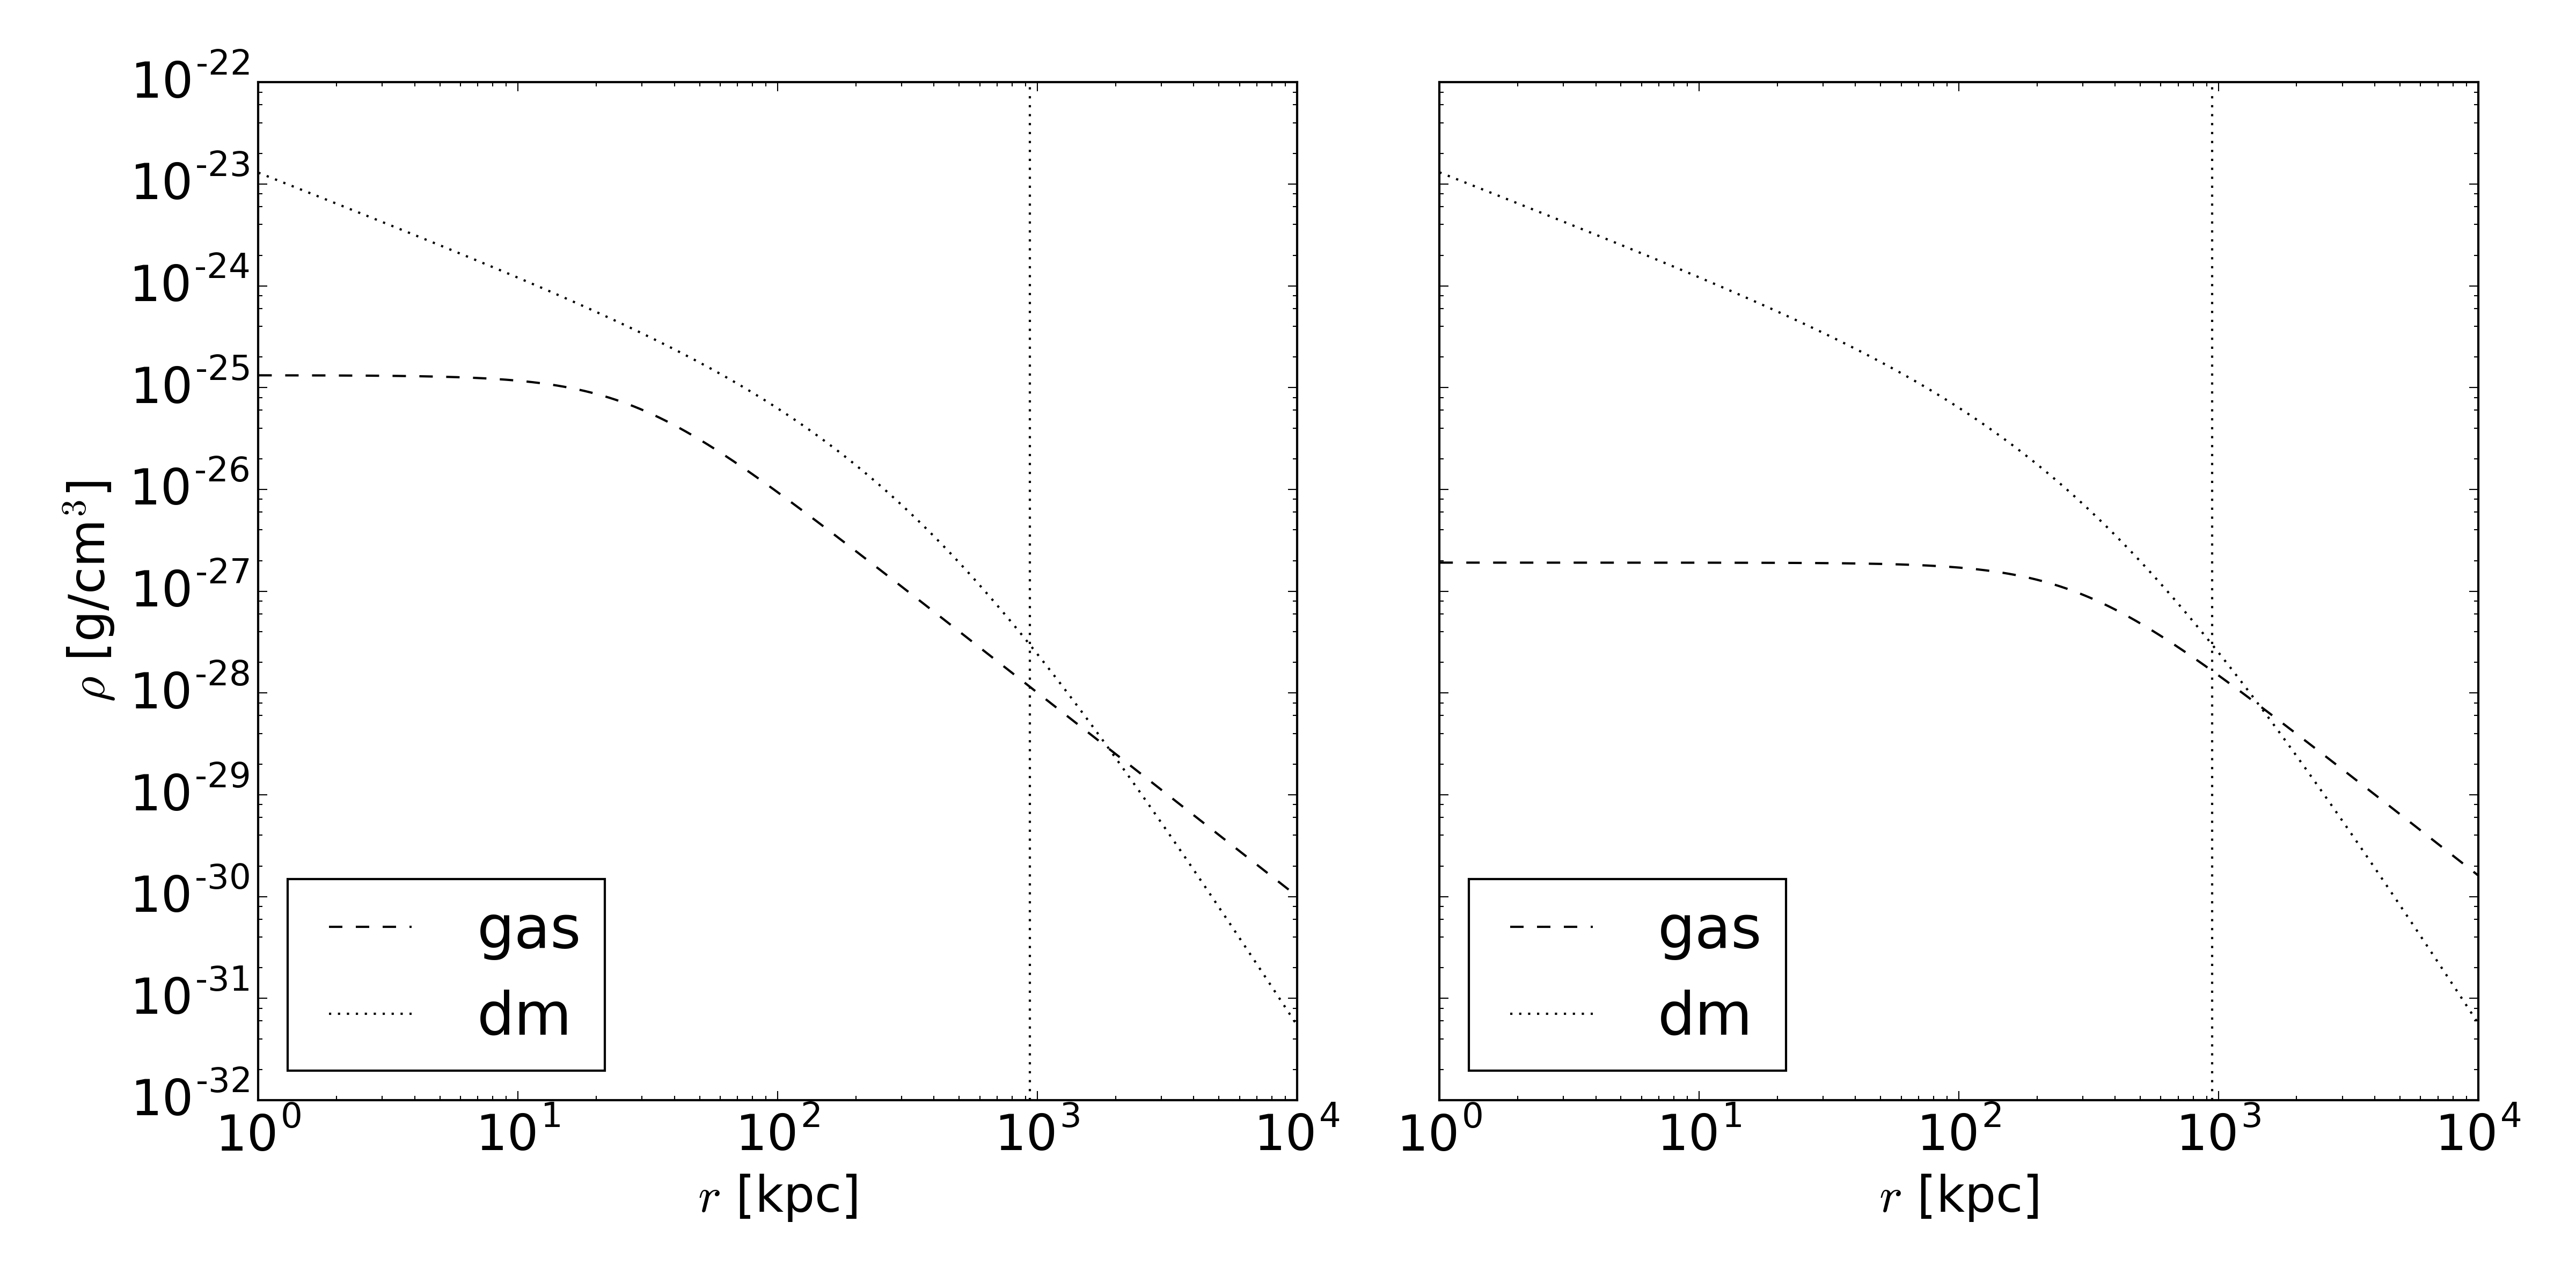
\includegraphics[width=\textwidth]{ics/cygA_cygNW_density.png}
%    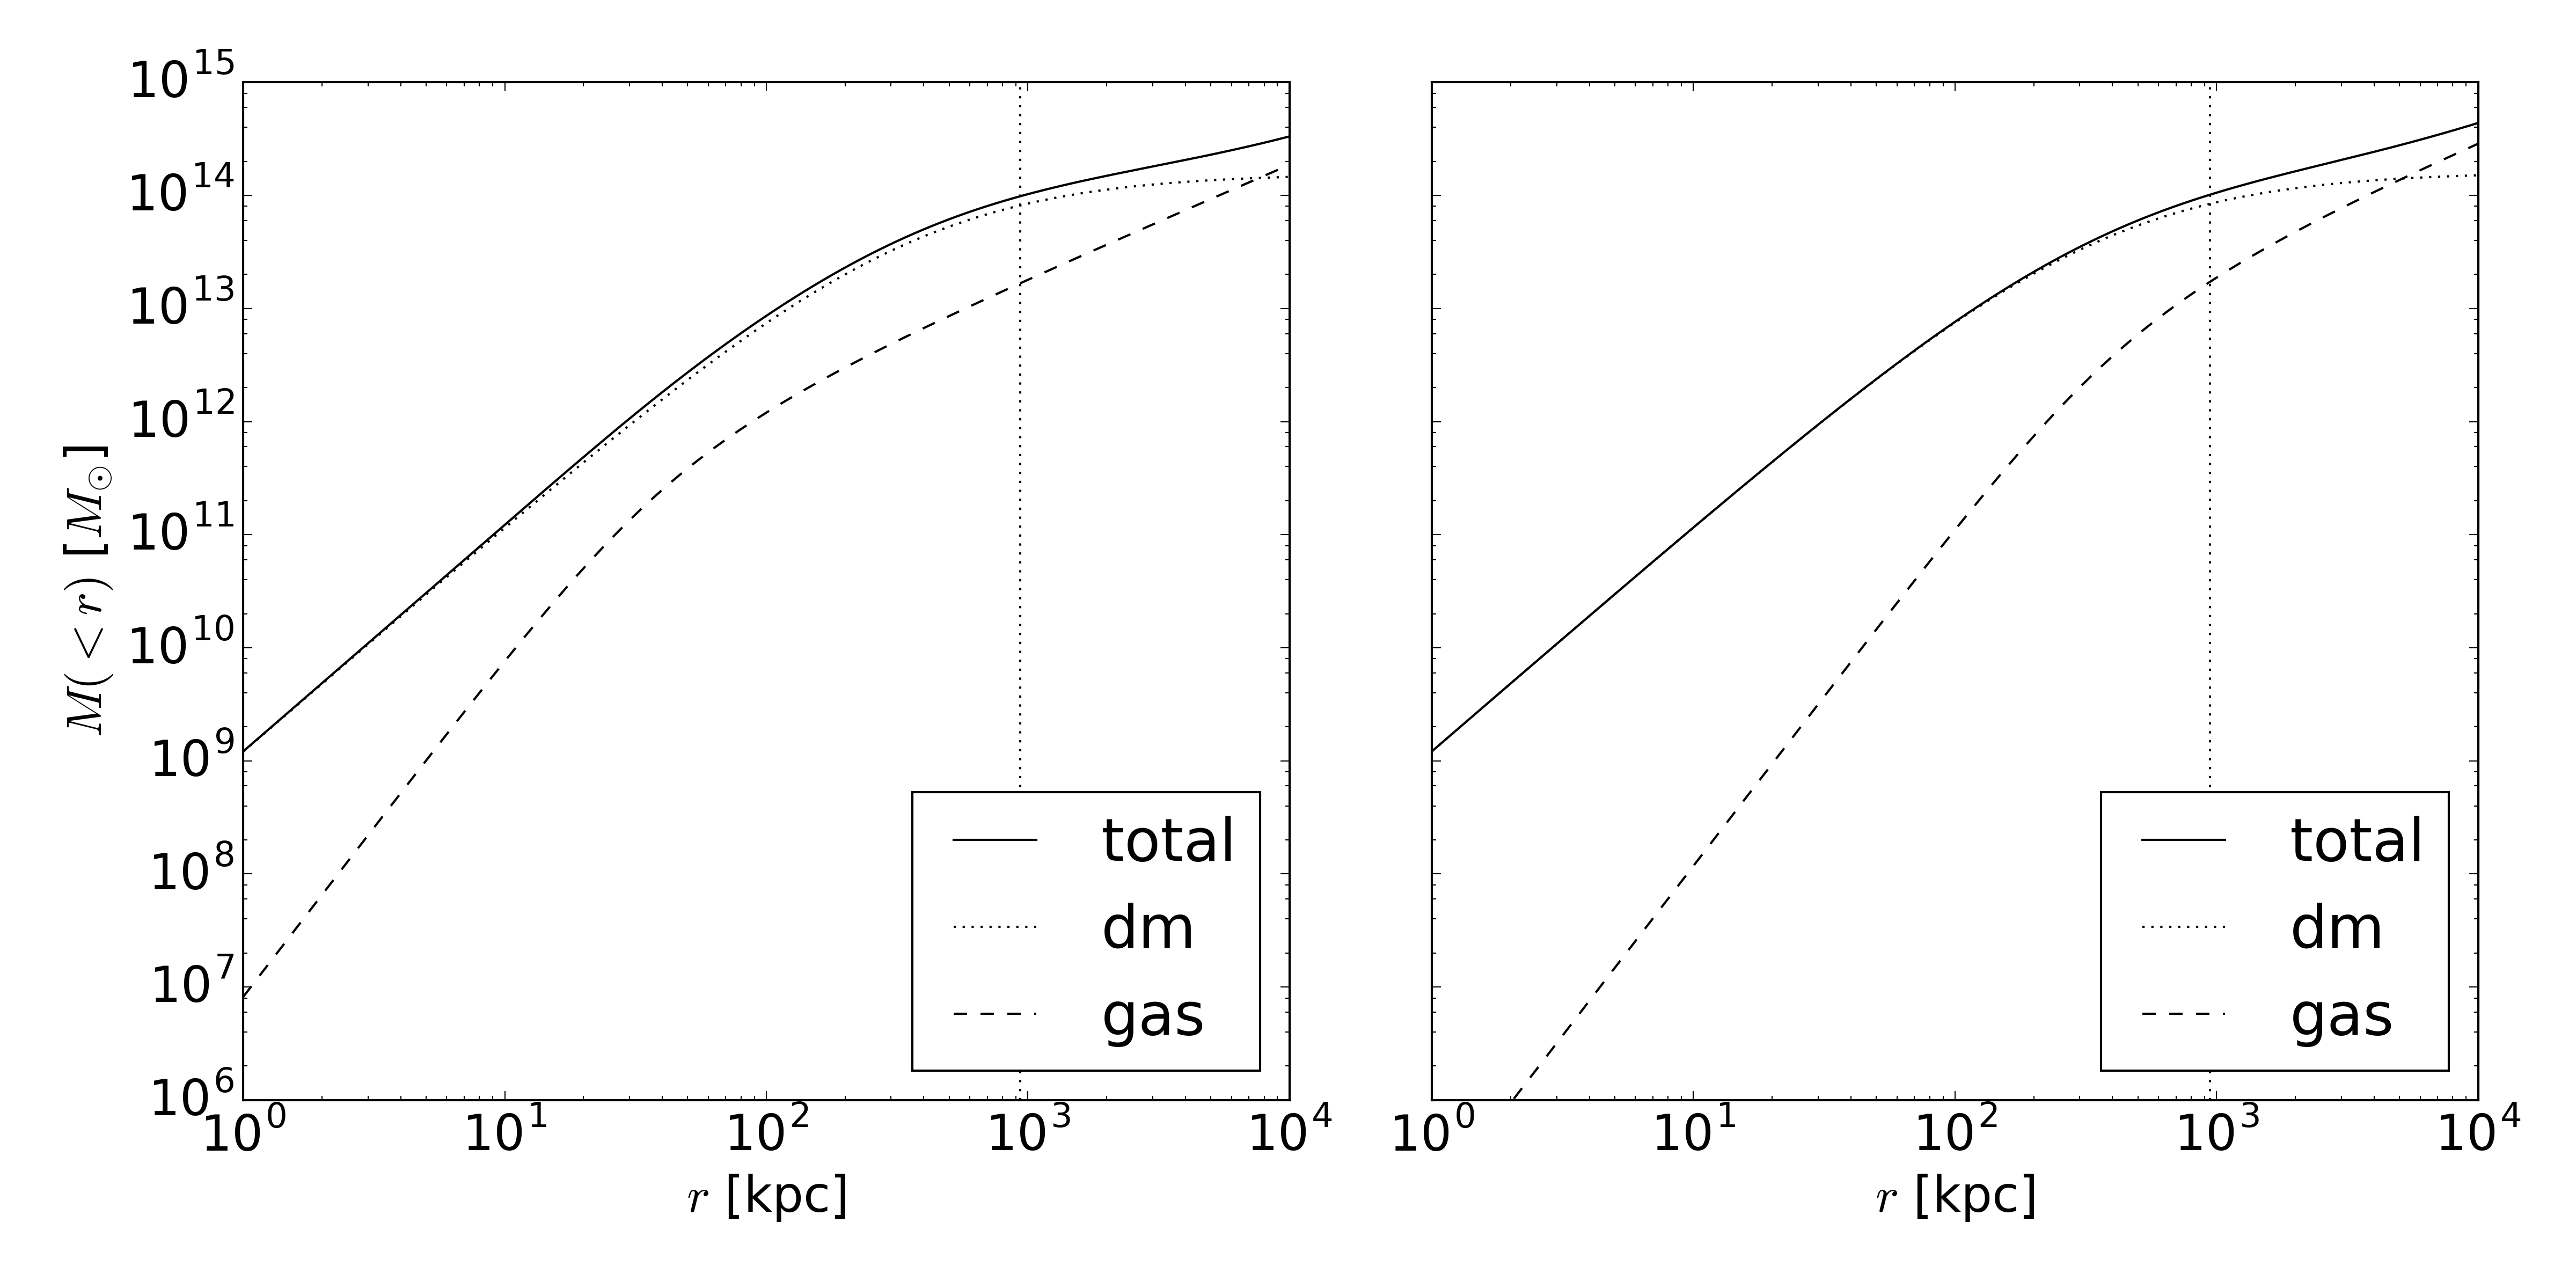
\includegraphics[width=\textwidth]{ics/cygA_cygNW_mass.png}
%    \caption{\emph{Top:} Radial density profiles of cygA (left), cygB (right).
%        \emph{Bottom:} Cumulative mass profile of cygA (left), cygB (right).
%        The vertical dotted line indicates $r_{200}$. The virial radii for
%        both sub clusters is equal, and the total gravitating mass is too.}
%    \label{fig:massAndDensity}
%\end{figure}
%\SubfileBibliography
%\end{document}


\begin{figure}[p]
    \centering
    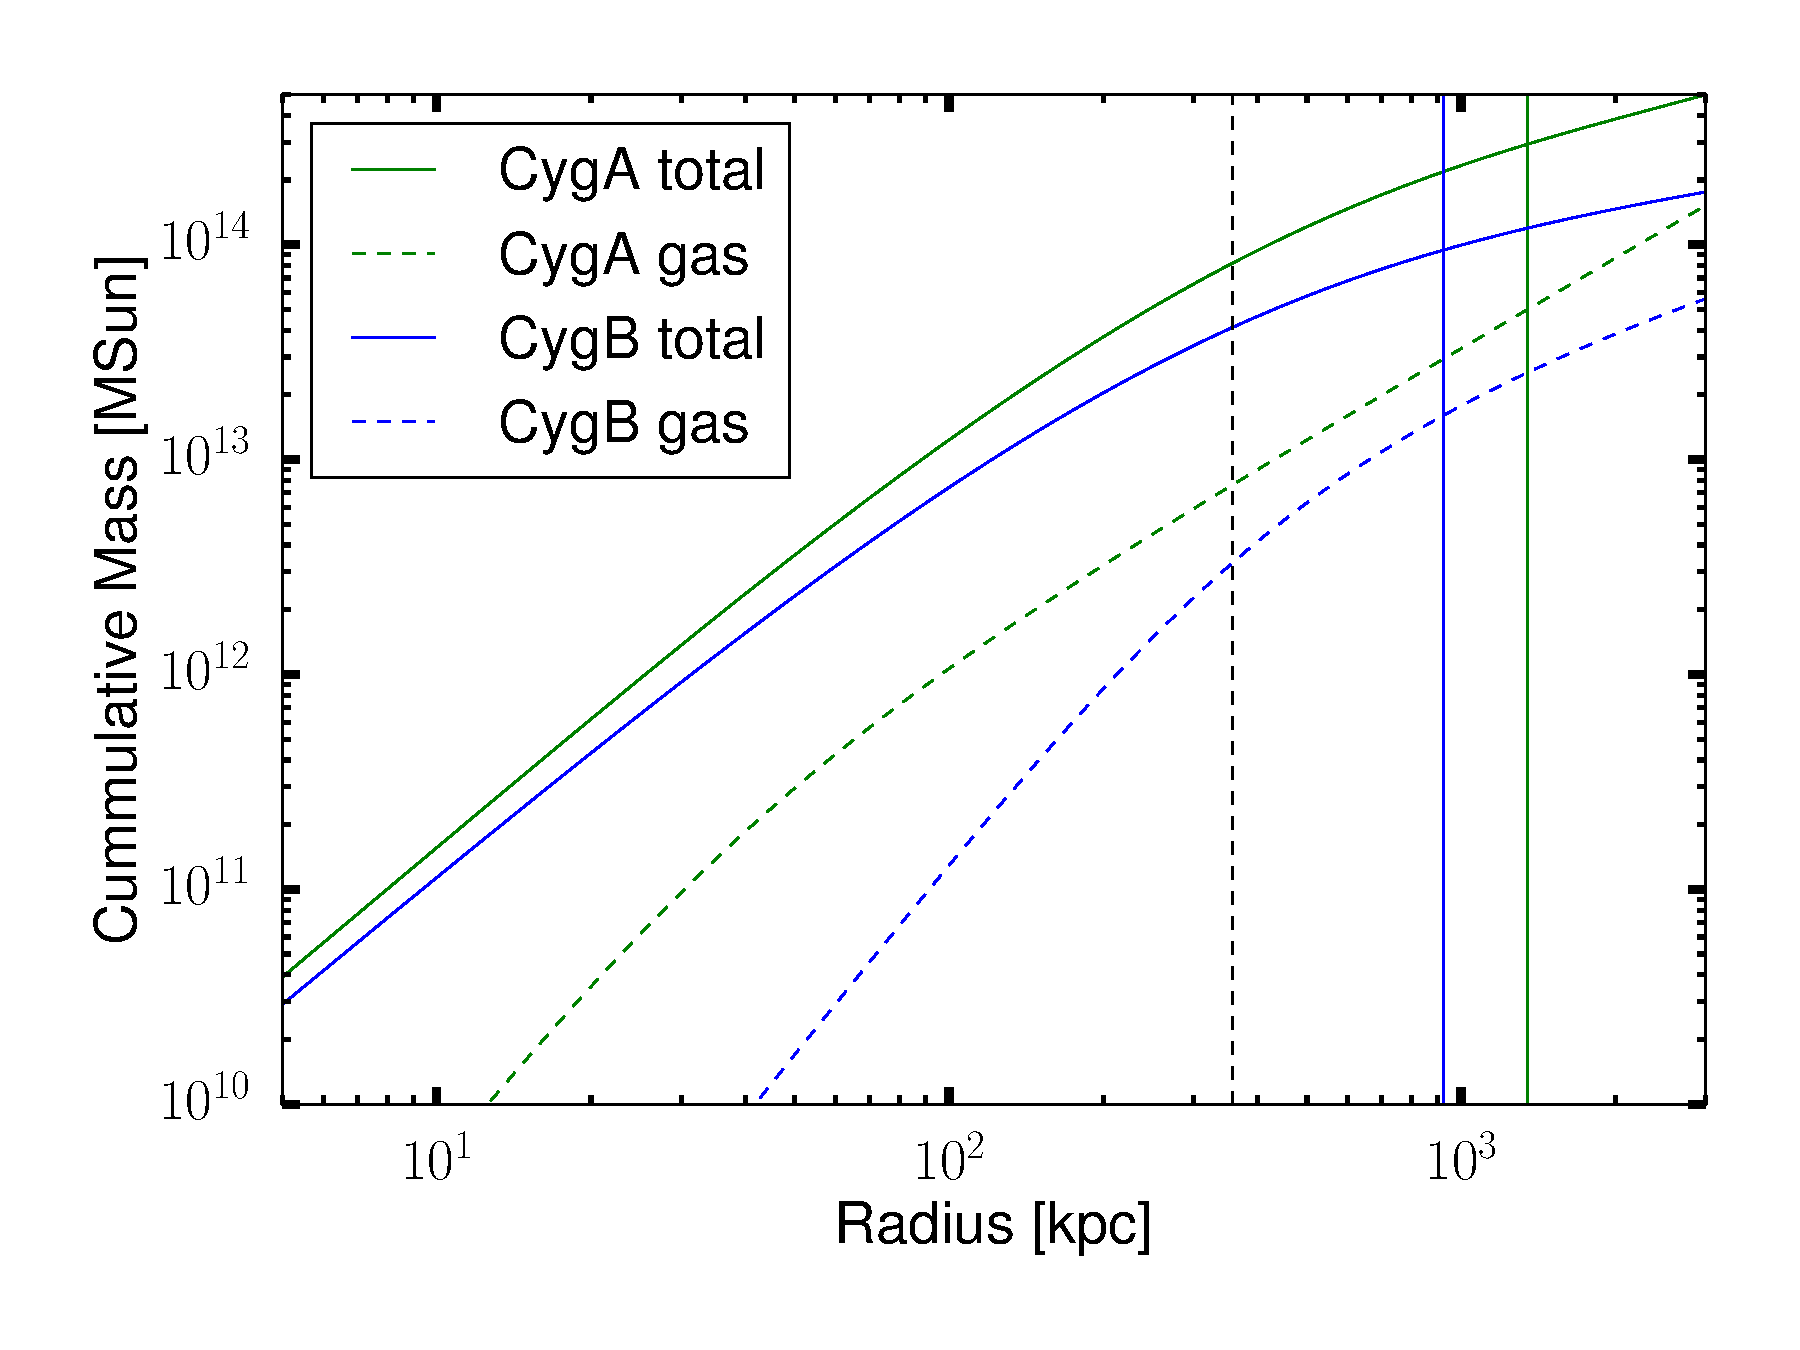
\includegraphics[width=0.9\textwidth]{ics/radial/cygA_cygB_mass_sameplot_freebeta_900ksec.pdf}
    \caption{Derived mass profile of CygA and CygB using the beta model where
             beta is left as a free parameter. The solid lines indicates the 
             total mass (baryonic plus dark matter). CygA is indicated by the
             green lines, while CygB is shown in blue. The visible and total
             gravitating mass differ significantly. The dashed black line 
             indicates 500 kpc when $H_0=50$ to guide the eye when comparing 
             our results to prior mass estimates \citep{2005AJ....130...47L}.
             The coloured solid vertical lines show the virial radii.}
    \label{fig:massAndDensity_freebeta}
    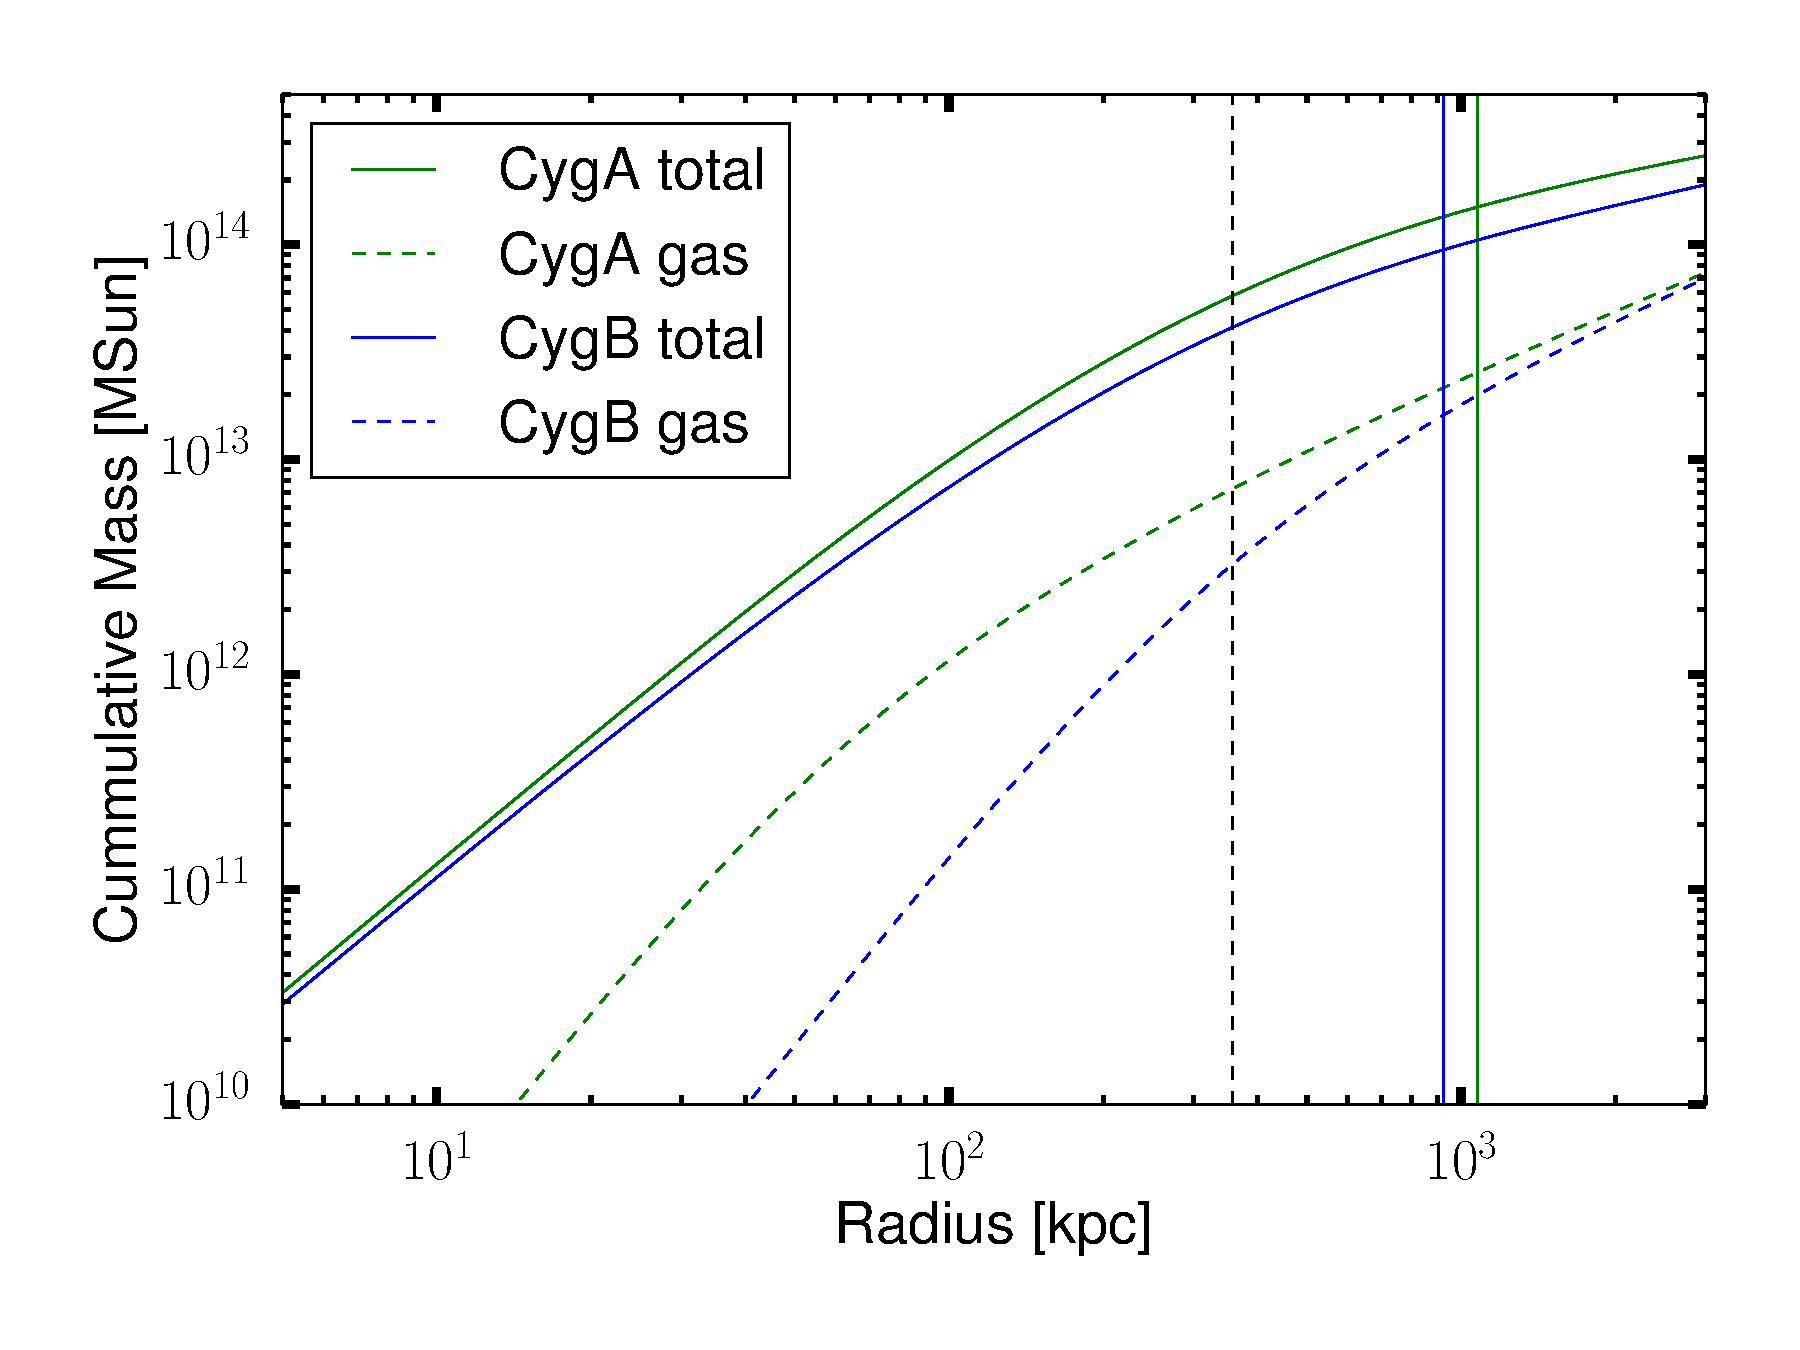
\includegraphics[width=0.9\textwidth]{ics/radial/cygA_cygB_mass_sameplot_900ksec.pdf}
    \caption{Derived mass profiles for $\beta = 2/3$.}
    \label{fig:massAndDensity_fixedbeta}
\end{figure}


\begin{figure}[p]
    \centering
    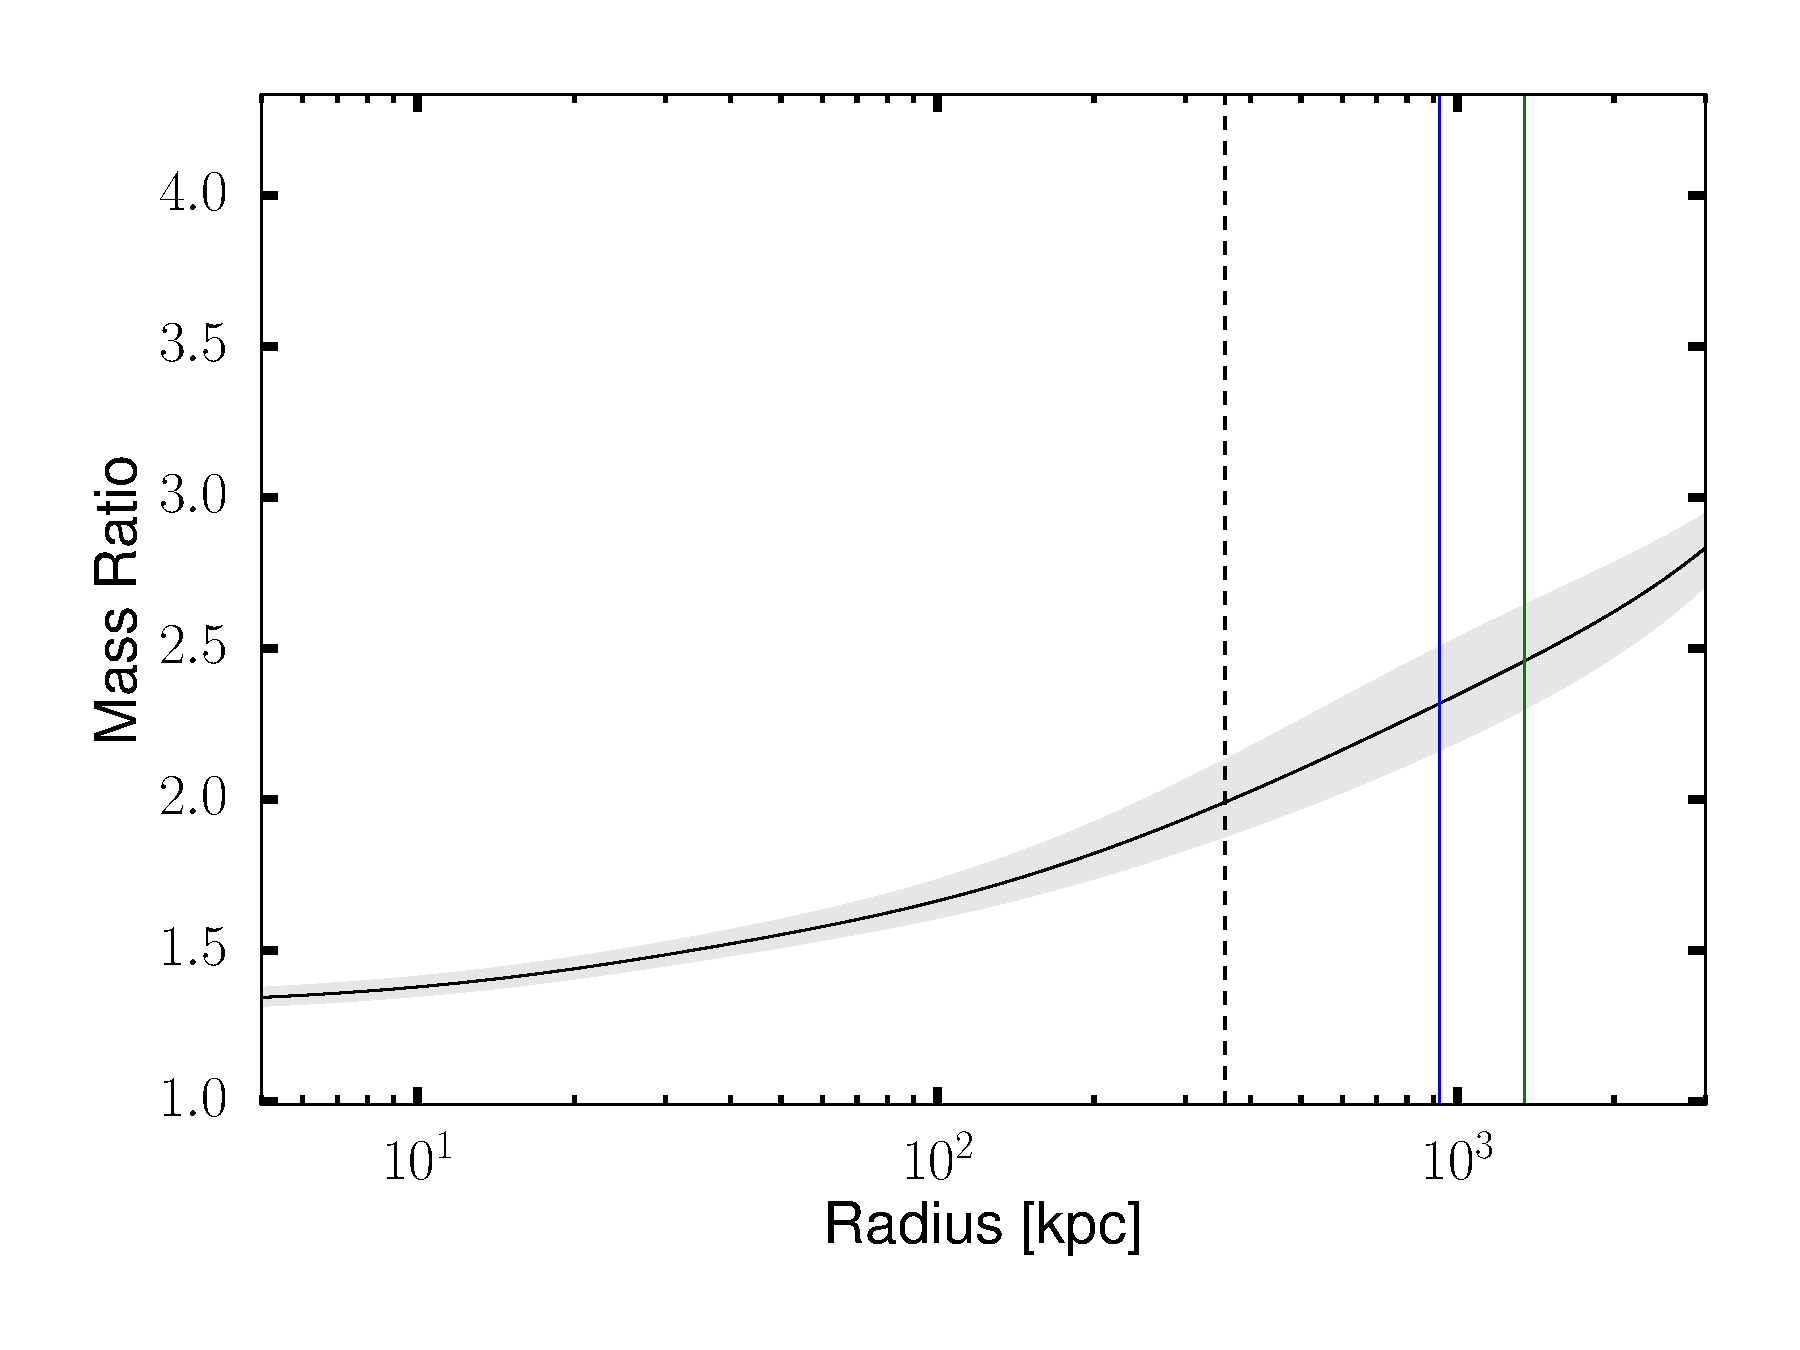
\includegraphics[width=0.9\textwidth]{ics/radial/cygA_cygB_massRatio_freebeta_900ksec.pdf}
    \caption{Derived mass ratio plot of the total gravitating mass as a function 
             of enclosing radius for the free-beta values. The shaded gray areas
             indicate the propagated uncertainties, and the green and blue vertical 
             lines show the virial radii of CygA, respectively CygB. The dashed 
             black line indicates 500 kpc when $H_0=50$ to guide the eye when comparing 
             our results to prior mass estimates \citep{2005AJ....130...47L}.
             }
    \label{fig:massRatio_feebeta}
    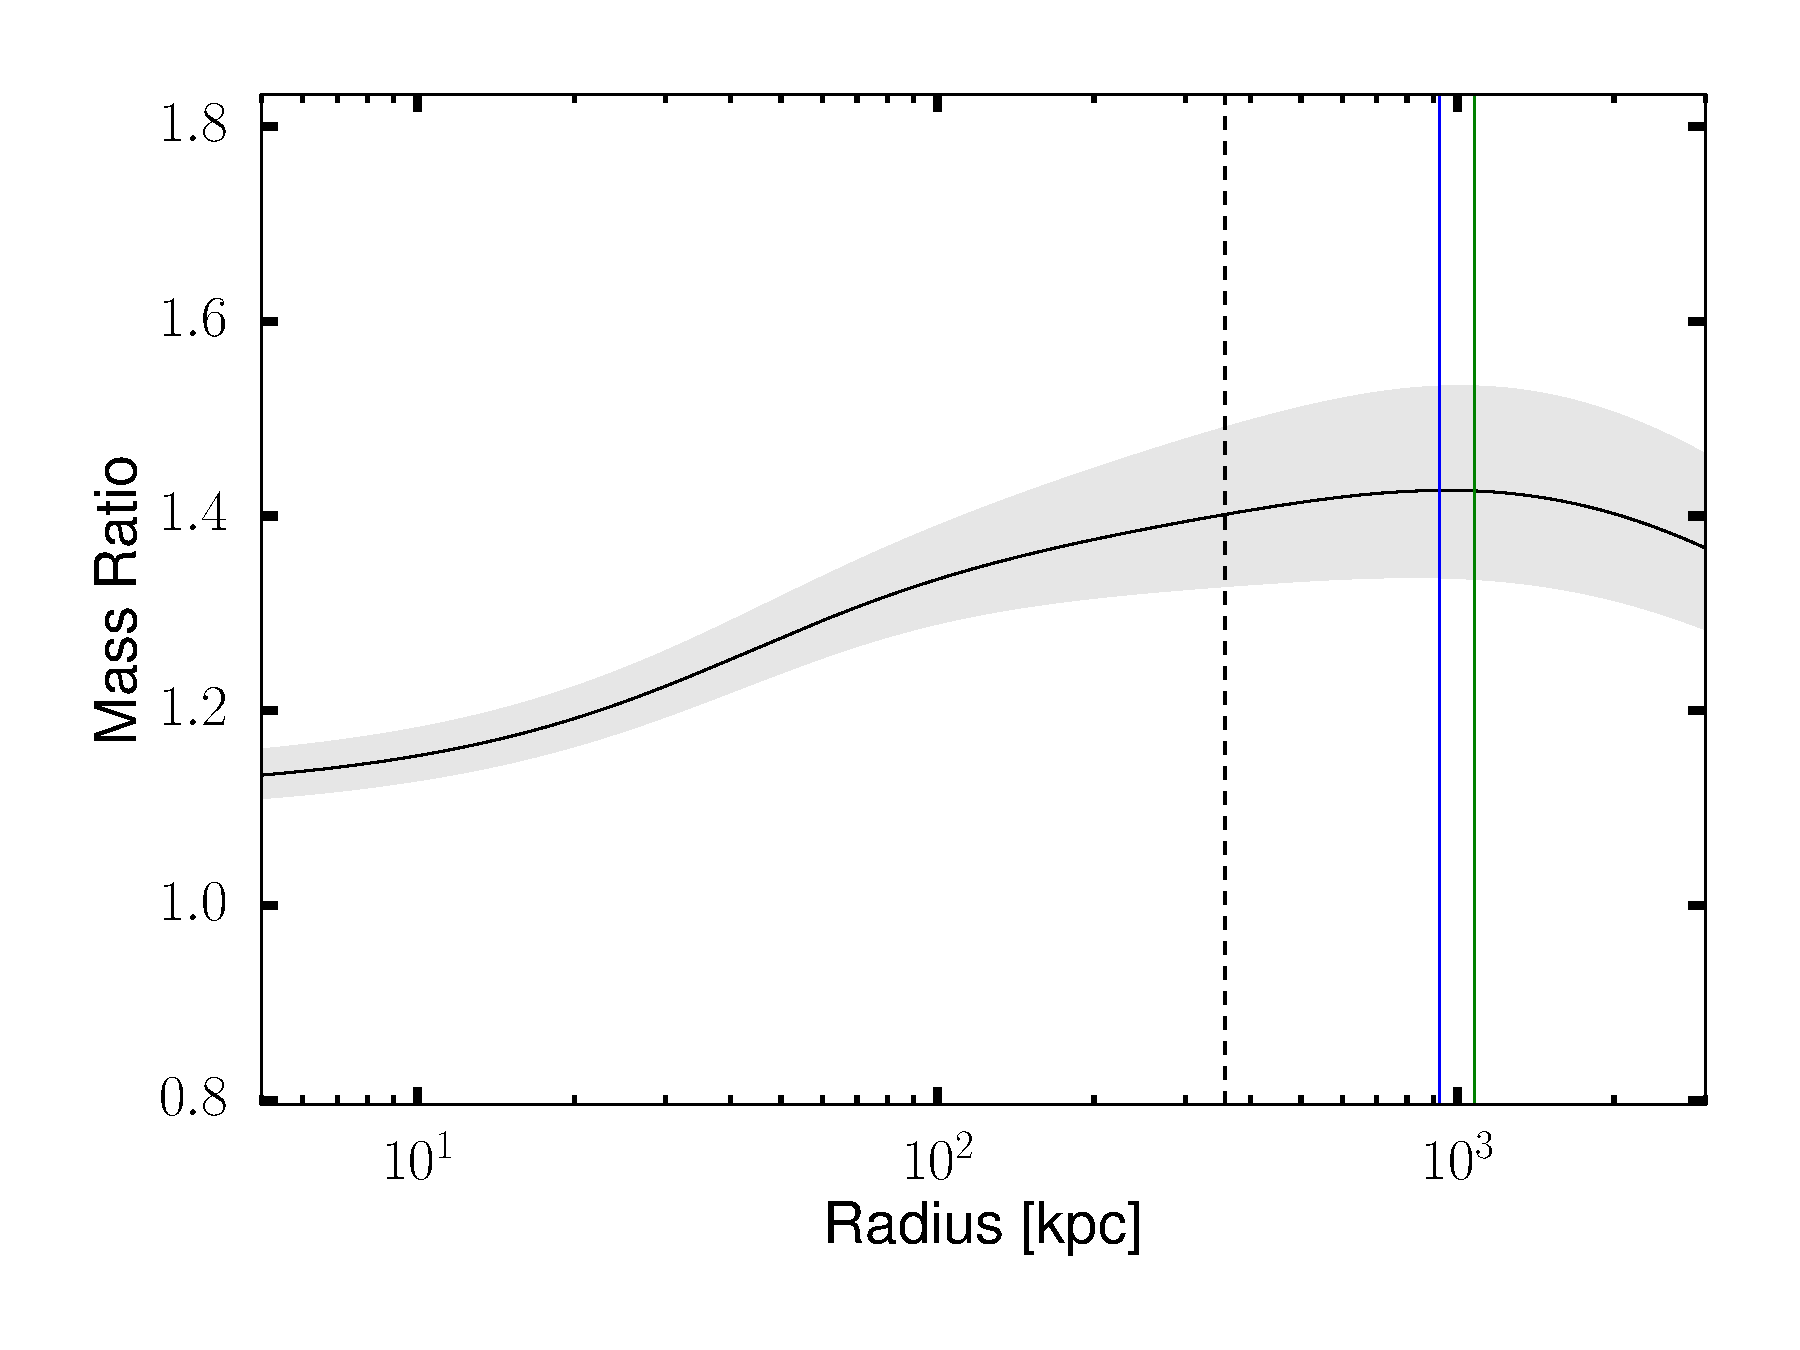
\includegraphics[width=0.9\textwidth]{ics/radial/cygA_cygB_massRatio_900ksec.pdf}
    \caption{Derived mass ratio for $\beta = 2/3$.}
    \label{fig:massRatio_feebeta}
\end{figure}





% \section*{The Baryon Fraction}
% \label{sec:theory-baryonfraction}
% TODO: include section about baryon fraction? \citep{2013MNRAS.431.1487P}


% \mycomment{Leave in, or discard?}
% \section{Statistics Model}
% \label{sec:theory-statistics}
% For sufficient photon counts in each individual bin, one can assume the errors
% in the bins follow the normal distribution, thus, given $n$ data points that
% are distributed independently the response data will have the distribution
% given by equation~\ref{eq:pdf_chisq}. We assume a count of 25 photons per bin
% suffices to ensure a normal distribution of errors within the bins according to
% central limit theorem. We adopt the following equations from
% \citet{2013scin.book.....V}.
% 
% TODO: add log likelihood and add proper description of how and when to reject
% TODO: add `Pearson'.
% null hypothesis. Maybe also add the steps: define H0, define test statistic,
% obtain observed value of test statistic, calculate chi2 pdf $p$-value, check
% if H0 accepted or rejected, set limits on when to reject/accept.
% \begin{align}
%     p(\boldsymbol{y}|\boldsymbol{\mu},\boldsymbol{\sigma}^2)
%     &= \sum\limits_{i=1}^{n} \frac{1}{\sqrt{2 \pi \sigma_i^2}}
%     \exp \left\{ - \frac{(y_i-\mu_i)^2}{\sigma_i^2} \right\}
%     \label{eq:pdf_chisq} \\
%     X^2(\boldsymbol{\theta}) &= -2 L(\boldsymbol{\theta}) + \text{const}
%     = \sum\limits_{i=1}^{n} \frac{(y_i-\mu_i)}{\sigma_i^2} \label{eq:chisq} ,
% \end{align}
% 
% \noindent where $\mu_i = E[y_i] = f(x_i, \boldsymbol{\theta})$ is a physics model
% depending on unknown parameters $\boldsymbol{\theta} = \{ \theta_1, ..., \theta_M\}$,
% $\boldsymbol{\sigma}^2$ is the variance, and $\boldsymbol{y}$ is are the measured
% values. We then minimise equation~\ref{eq:chisq} to maximise the log likelihood
% $L(\boldsymbol{\theta})$ to obtain the maximum likelihood estimates (MLEs),
% or `fit parameters'. We will use $\chi^2$ as symbol for the weighted least squares $X^2$.
% TODO: this is overkill? We can simply say `we use $\chi^2$', or `least-squares'
% fitting?


\newpage

\section{Radial Profiles: Temperature}
\label{sec:ChandraTemperature}

The \satellite{Chandra} observation is split up into four different wedges,
as shown in Figure~\ref{fig:wedges}.
\begin{enumerate}
    \item The merger region: A $90$-degree wedge centered on the merger axis, 
          from $6$ to $96$ degrees
    \item The cold region: A $90$-degree wedge center on the extended cold region,
          from $225$ to $315$ degrees
    \item The hot region: One wedge between $96$ and $225$ degrees and one wedge
          between $315$ and $366$ degrees, consisting of the hot gas not directly
          around the merger axis
    \item The average region: A $270$-degree wedge centered on the merger axis, 
          from $96$ to $6$ degrees
\end{enumerate}

The average and merger sectors have already been used in the extraction of the
number density. The merger wedge is cut-out, and the density profile is obtained
from the remaining area. Turning to the temperature profile, these two wedges 
are used to obtain the average and merger temperature structure. Moreover, 
two additional sectors are defined. By eye, the temperature appears hotter or
colder than average in certain regions. Figure~\ref{fig:wedges} shows how the 
two-dimensional projection of the X-ray surface brightness is divided up in 
the four regions. Note that the hot and cold regions are only defined for CygA. 
The average region is the combination of the merger, hot and cold region, but
because of the adaptive binning these three regions cannot simply be averaged.
The profiles of CygB are obtained from spherical wedges centered on CygB.
For each region a radial temperature profile is extracted and, again, we refer
to \citet[in prep]{2016MNRAS.123..456W} for the full details of the data analysis. 
Figure~\ref{fig:AdaptiveRadiiOfWedges} shows the radii within the wedges to
clarify the adaptive binning. The resulting temperature profiles are presented
in Figure~\ref{fig:ObservedWedgeProfiles}.



\begin{figure}
    \centering
    \makebox[\textwidth][c]{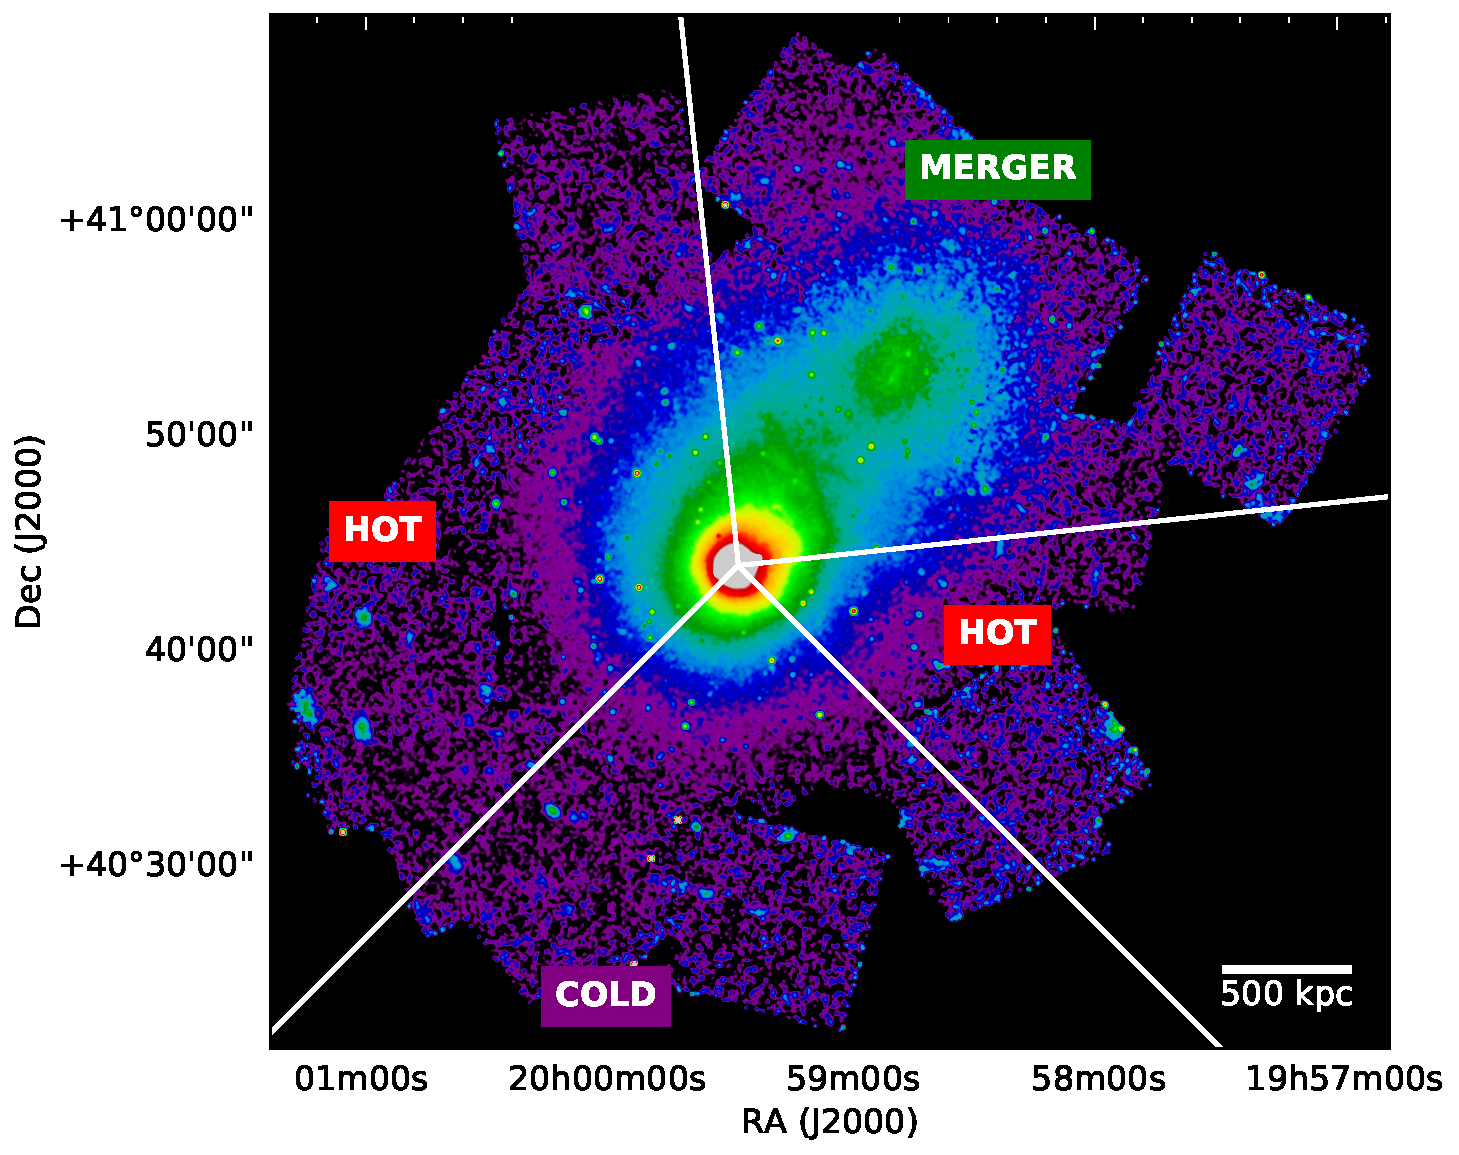
\includegraphics[width=1.3\textwidth]{ics/xray/mosaic_xray_wedges.pdf}}%
    \caption{Preliminary 982~ksec \satellite{Chandra} observation
             \citep[in prep]{2016MNRAS.123..456W} showing the CygA radial profile
             extraction regions overplotted on the full mosaic. The wedges are 
             from $6$\deg-$96$\deg \, (merger), $96$\deg$-225$\deg \, and
             $315$\deg-$366$\deg \, (hot), and $225$\deg-$315$\deg \, (cold).
             The `quiescent', or average profile spans $96$\deg-$366$\deg
             (not explicitly indicated here).}
    \label{fig:wedges}
\end{figure}


\begin{figure}
    \centering
    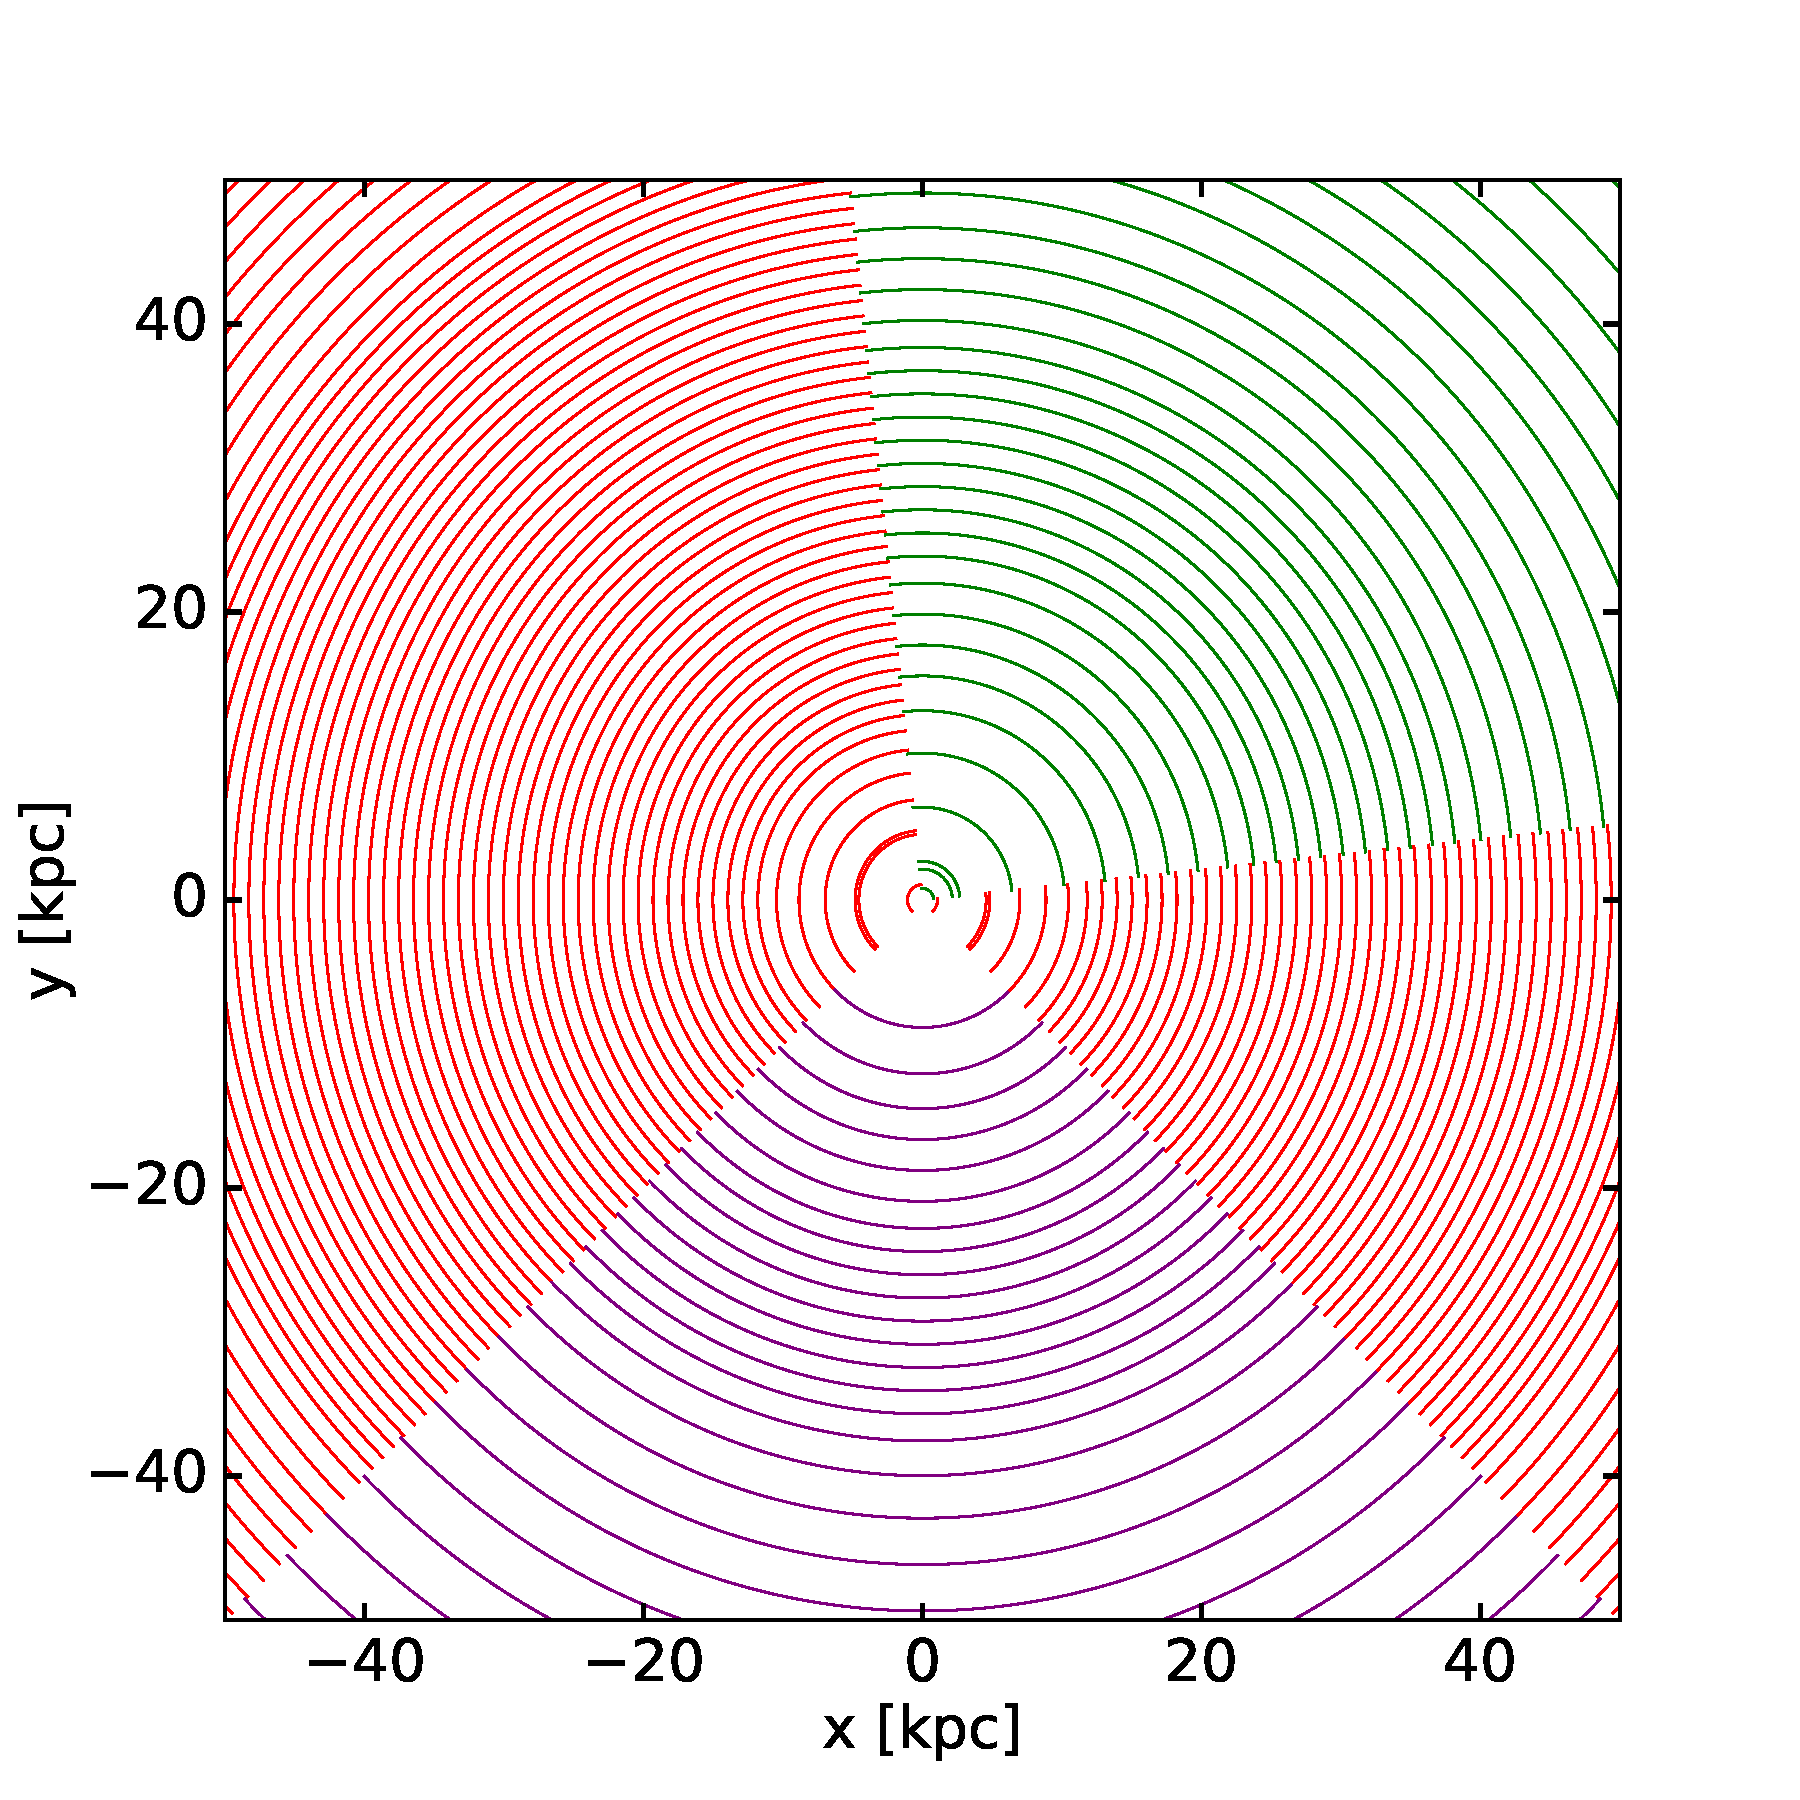
\includegraphics[width=0.5\textwidth]{ics/temperature/chandra_adaptivebinning_regions_50}
    \caption{The temperature profiles are obtained using an adaptive binning
             technique within wedges. This plot shows the central radii within 
             the wedges at which the observed data points are taken.}
    \label{fig:AdaptiveRadiiOfWedges}

    \makebox[\textwidth][c]{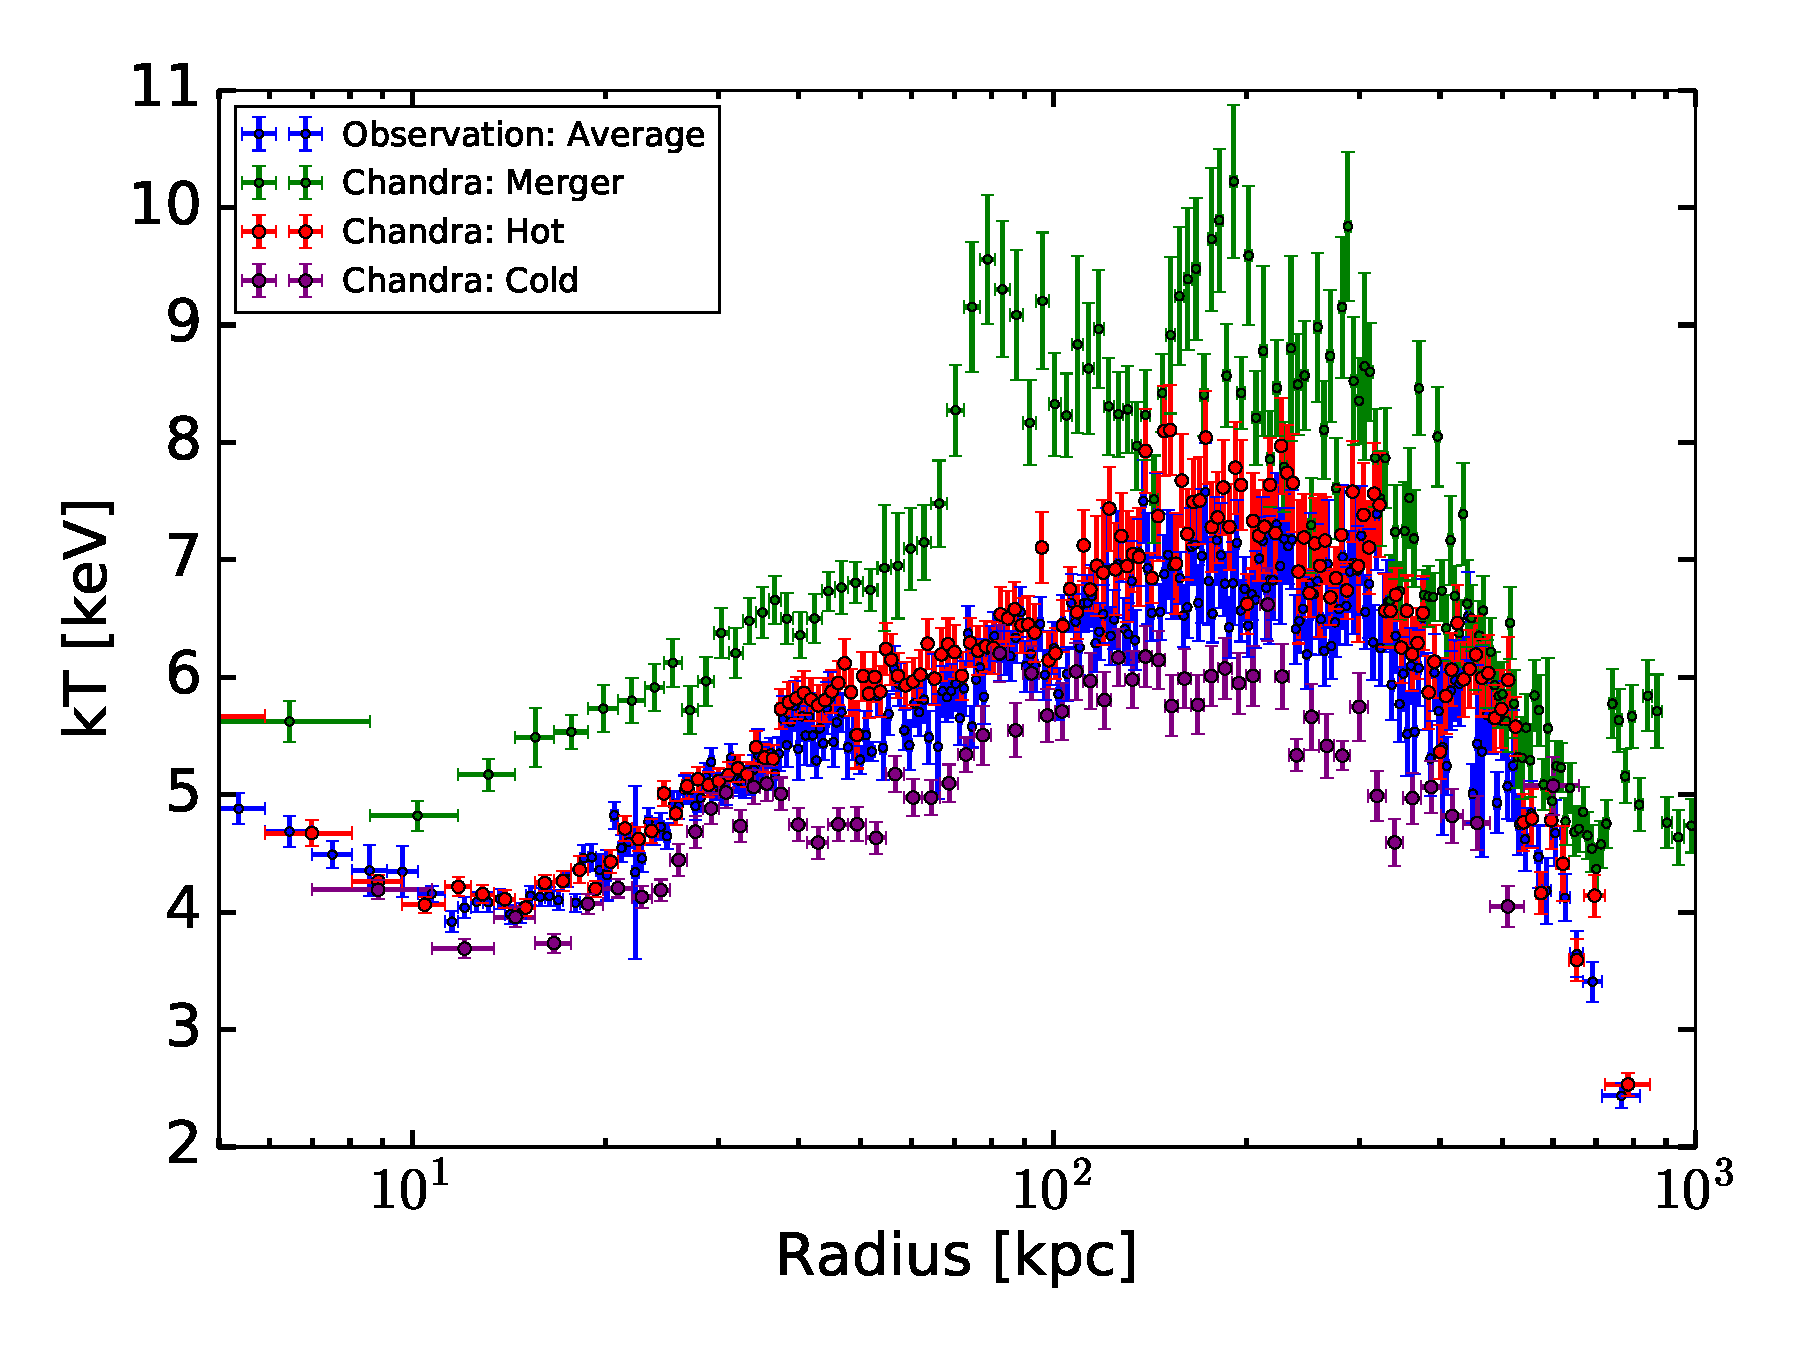
\includegraphics[width=1.3\textwidth]{ics/temperature/ObservedTemperatureStructure.pdf}}%
    \caption{Resulting radial temperature profiles extracted at the four wedges.
             Data courtesy of Martijn de Vries.}
    \label{fig:ObservedWedgeProfiles}
\end{figure}



\SubfileBibliography
\end{document}
